% Options for packages loaded elsewhere
%\PassOptionsToPackage{unicode}{hyperref}
\PassOptionsToPackage{hyphens}{url}
%
\documentclass[11pt]{article}
\usepackage{indentfirst}
\usepackage{placeins}
\usepackage{lmodern}
\usepackage{amssymb,amsmath,,amsfonts,amsthm}
\newtheorem*{remarque}{Remarque}
\usepackage{ifxetex,ifluatex}
\ifnum 0\ifxetex 1\fi\ifluatex 1\fi=0 % if pdftex
  \usepackage[T1]{fontenc}
  \usepackage[utf8]{inputenc}
  \usepackage{textcomp} % provide euro and other symbols
\else % if luatex or xetex
  \usepackage{unicode-math}
  \defaultfontfeatures{Scale=MatchLowercase}
  \defaultfontfeatures[\rmfamily]{Ligatures=TeX,Scale=1}
\fi
% Use upquote if available, for straight quotes in verbatim environments %
\IfFileExists{upquote.sty}{\usepackage{upquote}}{}
\IfFileExists{microtype.sty}{% use microtype if available
  \usepackage[]{microtype}
  \UseMicrotypeSet[protrusion]{basicmath} % disable protrusion for tt fonts
}{}
\makeatletter
\@ifundefined{KOMAClassName}{% if non-KOMA class
  \IfFileExists{parskip.sty}{%
    \usepackage{parskip}
  }{% else
    \setlength{\parindent}{0pt}
    \setlength{\parskip}{6pt plus 2pt minus 1pt}}
}{% if KOMA class
  \KOMAoptions{parskip=half}}
\makeatother
\usepackage{xcolor}
\IfFileExists{xurl.sty}{\usepackage{xurl}}{} % add URL line breaks if available
%\IfFileExists{bookmark.sty}{\usepackage{bookmark}}{\usepackage{hyperref}}
\urlstyle{same} % disable monospaced font for URLs
\usepackage[margin=1in]{geometry}
\usepackage{color}
\usepackage{fancyvrb}
\newcommand{\VerbBar}{|}
\newcommand{\VERB}{\Verb[commandchars=\\\{\}]}
\DefineVerbatimEnvironment{Highlighting}{Verbatim}{commandchars=\\\{\}}
% Add ',fontsize=\small' for more characters per line
\usepackage{framed}
\usepackage{changepage}
\usepackage{graphicx,grffile}
\makeatletter
\def\maxwidth{\ifdim\Gin@nat@width>\linewidth\linewidth\else\Gin@nat@width\fi}
\def\maxheight{\ifdim\Gin@nat@height>\textheight\textheight\else\Gin@nat@height\fi}
\makeatother
% Scale images if necessary, so that they will not overflow the page
% margins by default, and it is still possible to overwrite the defaults
% using explicit options in \includegraphics[width, height, ...]{}
\setkeys{Gin}{width=\maxwidth,height=\maxheight,keepaspectratio}
% Set default figure placement to htbp
\makeatletter
\def\fps@figure{htbp}
\makeatother
\setlength{\emergencystretch}{3em} % prevent overfull lines
\providecommand{\tightlist}{%
  \setlength{\itemsep}{0pt}\setlength{\parskip}{0pt}}
%\setcounter{secnumdepth}{-\maxdimen} % remove section numbering
%C'est fini pour les packages pour le code R
\usepackage[francais]{babel}
\usepackage[T1]{fontenc}
\usepackage{a4wide}

% \usepackage{biblatex} %Imports biblatex package
\usepackage[backend=biber,style=authoryear,citetracker=true,natbib=true]{biblatex}
\addbibresource{./bibliographie/sample.bib} %Import the bibliography file

\pagestyle{myheadings}
\usepackage{fancyhdr}
\usepackage{amsmath,amsfonts,amssymb}
\pagestyle{plain}
\usepackage{subcaption}
\usepackage{xcolor}
\usepackage{mdframed}
\usepackage{color,soul}
\sethlcolor{yellow}
\pagestyle{fancy}
%\fancyhead[C]{\thechapter}
%\fancyhead[CE]{contenu}
%\fancyfoot[c]{\thepage}
\renewcommand{\headrulewidth}{1pt}
%\fancyhead[C]{ }
\fancyhead[L]{Classification supervisée de personnages}
\renewcommand{\footrulewidth}{1pt}
\fancyfoot[C]{\textbf{\thepage}}
\fancyfoot[L]{ Master 1 -- MIND}
\fancyfoot[R]{ 2020/2021}

%\usepackage{float}
\usepackage{mathtools}
%\usepackage{algorithm}
\usepackage[]{algorithmic}
\usepackage{algorithm2e}
%--
%setcounter{secnumdepth}{4}
%\newcommand{\myparagraph}[1]{\paragraph{#1}\mbox{}\\}
%\documentclass[12pt]{book}
\usepackage[utf8]{inputenc}
%\usepackage[frenchb]{babel}
%\usepackage{lipsum}
\usepackage{graphics}
\usepackage{graphicx}
\usepackage{xcolor, soul}
\sethlcolor{yellow}
\usepackage[french]{minitoc}
\usepackage[colorlinks = true,
            linkcolor = blue,
            urlcolor  = black,
            citecolor = black]{hyperref}
%\usepackage{minitoc}

\usepackage{float}
\usepackage[textwidth=1.5cm, textsize=scriptsize]{todonotes}
%\newcommand{\tif}[1]{\todo[color=blue!20]{\textbf{ Tif:} #1}}
\usepackage{./shortcut}
\DeclareMathOperator{\vote}{Vote Majoritaire}
\usepackage{ulem} % ne pas le supprimer !!!!!
\begin{document}
\thispagestyle{empty}
\begin{titlepage}
  \begin{sffamily}
  \begin{center}

    % Upper part of the page. The '~' is needed because \\
    % only works if a paragraph has started.





    % Title

    
\includegraphics[width= 10 cm]{./figures/untitled.png}
    \\[3cm]
    \textsc{Master 1 MIND }\\
    \vspace{0.4cm}
    \textsc{Rapport de projet }\\
    \vspace{1cm}

    \hrule
    \vspace{0.4cm}
    { \huge \scshape \textbf{Classification supervisée de personnages sur la saga Harry Potter}}
    \vspace{0.4cm}
    \hrule
    \vspace{4 cm}



    % Author and supervisor
    \begin{minipage}{0.5\textwidth}
      \begin{flushleft} \Large
        \emph{Auteurs : }\\
        \textsc{Bouthayna HAYOU}\\
        \textsc{Jihène BELGAIED }\\
        \textsc{Jalal SAKHER}\\

      \end{flushleft}
    \end{minipage}
    \begin{minipage}{0.43\textwidth}
      \begin{flushright} \Large
        \emph{Encadrants : }\\
    \textsc{Florent BASCOU}\\
    \textsc{Tiffany CHERCHI}
      \end{flushright}
    \end{minipage}

    \vfill

  \end{center}
  \end{sffamily}
\end{titlepage}

\newpage


\thispagestyle{plain} % empty
\mbox{}

\renewcommand{\contentsname}{Sommaire}
\tableofcontents
\newpage

\section{Introduction}

\tiff{Je vous conseille de commencer par décrire dès le début l'univers du film : c'est une saga sur un garçon qui découvre le fait que des sorcières et sorciers existent, et qu'il en fait partie. Il va dans une école de sorciers appelée Poudlard, où les étudiants sont classés dans ce qu'on appelle des "maisons". Ses aventures sont décrites dans XX films. Notre objectif est d'essayer de prédire l'appartenance d'un nouveau personnage à l'une des 4 maisons de Poudlard. Pour cela,}
Nous exploitons dans ce projet des données issues des 3 premières films de la saga Harry Potter à savoir « Harry Potter et la maison de sorciers », « Harry Potter et la Chambre des Secrets », « Harry Potter et le prisonnier d'Azkaban » ainsi qu'un dataframe donnant différentes caractéristiques des personnages; caractéristiques que nous décrieront par la suite.\\
Ajouter
L'objectif est de répondre à la question suivante : est-il possible de prédire appartenance d'un nouveau personnage à l'une des 4 maisons Poudlard ?

\tiff{Quel contexte, quelle problématique (cf commentaire), quelles pré-traitement des données, quelles méthodes statistiques, quelles difficultés statistiques.
Penser à faire une introduction globale. Vous pouvez déjà répondre au premier point. \\
L'introduction doit être "auto-suffisante" : on doit pouvoir comprendre tout le contexte et savoir tout ce que vous avez fait.}

Rajouter dans intro : les script des trois films seront préparés de la même façon. Par contre, pour la suite, nous utiliseront les script des 2 premiers pour entraîner notre modèle pour ensuite le tester sur le troisième.

\newpage

%------------------------------------------------------%
%------------------------------------------------------%
\section{Préparation des données}
%------------------------------------------------------%
%------------------------------------------------------%

La préparation de données est une étape étape primordiale dans le traitement de texte. En effet, elle a pour but de rendre les données textuelles brutes exploitables par l'ordinateur via de multiples opérations de nettoyage et transformation de texte que nous décrirons par la suite.\par

%------------------------------------------------------%
\subsection{Présentation des données}
%------------------------------------------------------%
\tiff{NON, cette présentation ne correspond pas au titre du projet proposé. Les données qui vous ont été données sont des tableaux qui contiennent deux colonnes : la première correspond au nom d'une personnage, la seconde à sa réplique. C'est tout. Et ENSUITE on ajoute des caractéristiques. Enfin, vous n'aviez pas besoin d'avoir ces données supplémentaires pour expliquer les différentes maisons et les différents statuts de sangs, etc. \\
 La seule feature supplémentaire nécessaire pour répondre à la question statistique du projet, c'était la variable "maison", qui est la réponse à prédire. Aucune des autres variables que vous utilisez dans ce dataframe était nécessaire. Ce projet concerne LES SCRIPTS.}


Dans le cadre de ce projet, nous utilisons des données collectées de plusieurs sources sur les trois premiers films de la saga Harry Potter. Ces données sont réparties sous forme de fichiers csv comme suivent:

\begin{itemize}
\renewcommand{\labelitemi}{$\bullet$}
    \item \textbf{Harry Potter 1, 2 et 3 :} ces données sont récupérées à partir des sous-titrages des films et sont divisées en deux colonnes : la première contenant les noms des personnages prenant la parole et la deuxième fournissant le discours du personnage correspondant divisé en phrase. Elles seront traitées par différentes techniques afin d'en construire des variables explicatives.

    \item \textbf{Characters :} ces données sont collectées de \cite{1} et \cite{2}. Elles décrivent les personnages des films en se basant principalement sur la  maison (Gryffindor, Ravenclaw, etc.), le sexe, le statut de sang, la loyauté et les compétences. Ces caractéristiques peuvent être utlisées comme variables additionnelles dans notre matrice de design.
\end{itemize}

Dans toute la suite de l'étude, nous séparerons les données du script en deux parties. La première étant celle correspondant au deux premiers films, et la deuxième, au troisième film.

%------------------------------------------------------%
\subsection{Prétraitement des scripts}
%------------------------------------------------------%

Dans un premier temps, nous examinons les données importées afin de corriger d’éventuelles erreurs liées à l'importation de données textuelles. En effet nous avons décelé bon nombre de caractères spéciaux, que nous avons supprimés ou remplacer afin d'éviter les erreurs dûes à la non compréhension par le langage Python durant la deuxième phase.\par

Dans un second temps, nous nous attardons sur le traitement numérique du langage (NLP: Natural Language Processing) qui consiste à traiter les scripts des films afin de les rendre exploitables par l'ordinateur. Cette opération est effectuée à l'aide du package python NLTK (Natural Language Toolkit), et est divisée en trois étapes :

\begin{itemize}
    \renewcommand{\labelitemi}{$\bullet$}
    \item \textbf{Tokenization :} La tokenisation consiste à découper un texte en morceaux. Ces morceaux pourraient être des phrases, des symboles ou des mots. C’est cette dernière option que l’on va choisir car nous elle nous permet de travailler directment sur les mots eux-mêmes. (plus simple pour retirer les stop words mais surtout pour mener à bien notre analyse statistique en seconde partie.)\par
    Exemple : "Here he comes, the birthday boy." $\Rightarrow ['here', 'he', 'comes', 'the', 'birthday', 'boy']$.

    \item \textbf{Stemming :} Afin de réduire la complexité d’un texte, on peut tirer parti de « classes d’équivalence »; on peut considérer que différentes formes d’un même mot (pluriel, singulier, conjugaison) sont équivalentes et les remplacer par une même forme dite canonique. Il existe deux approches dans le domaine:

        \begin{itemize}
            \renewcommand{\labelitemii}{-}
            \item La racinisation est simple à mettre en œuvre car elle peut s’appuyer sur des règles simples pour extraire la racine d’un mot, c’est-à-dire, le tronquer de toute déclinaison, accords et dérivations. Mais cette approche a ses défauts puisqu’elle peut changer les noms des personnages (Harry/Harri).

            \item La lemmatisation requiert la connaissance des statuts grammaticaux (exemple : chevaux devient cheval).
        \end{itemize}

    On fait donc le choix de la lemmatisation dans notre méthodologie, qui consiste à ramener un terme, quelque soit ses accords et déclinaisons à sa forme la plus simple. Cette méthode nous permettra d'avoir moins d'erreurs d'interprétation par la suite.\par
    Exemple : $['here', 'he', 'comes', 'the', 'birthday', 'boy'] \Rightarrow ['here', 'he', 'come', 'the', 'birthday', 'boy']$.

    \item \textbf{stop-words removal :} Cette étape consiste à enlever les mots communs comme les pronoms, prepositions, conjonctions, etc. qui n'apportent pas de valeur informative quant à la compréhension du "sens" du texte.\par
    Exemple : $['here', 'he', 'come', 'the', 'birthday', 'boy'] \Rightarrow ['birthday', 'boy']$.
\end{itemize}

%------------------------------------------------------%
\subsection{Visualisation et analyse de données}
%------------------------------------------------------%

Dans cette partie, nous exploitons les résultats obtenus de la partie prétraitement afin d'étudier et d'extraire les variables explicatives qui influencent principalement sur notre variable cible, dans ce cas l’appartenance à une maison Poudlard.\par

\begin{figure}[hbt!]
    \centering
    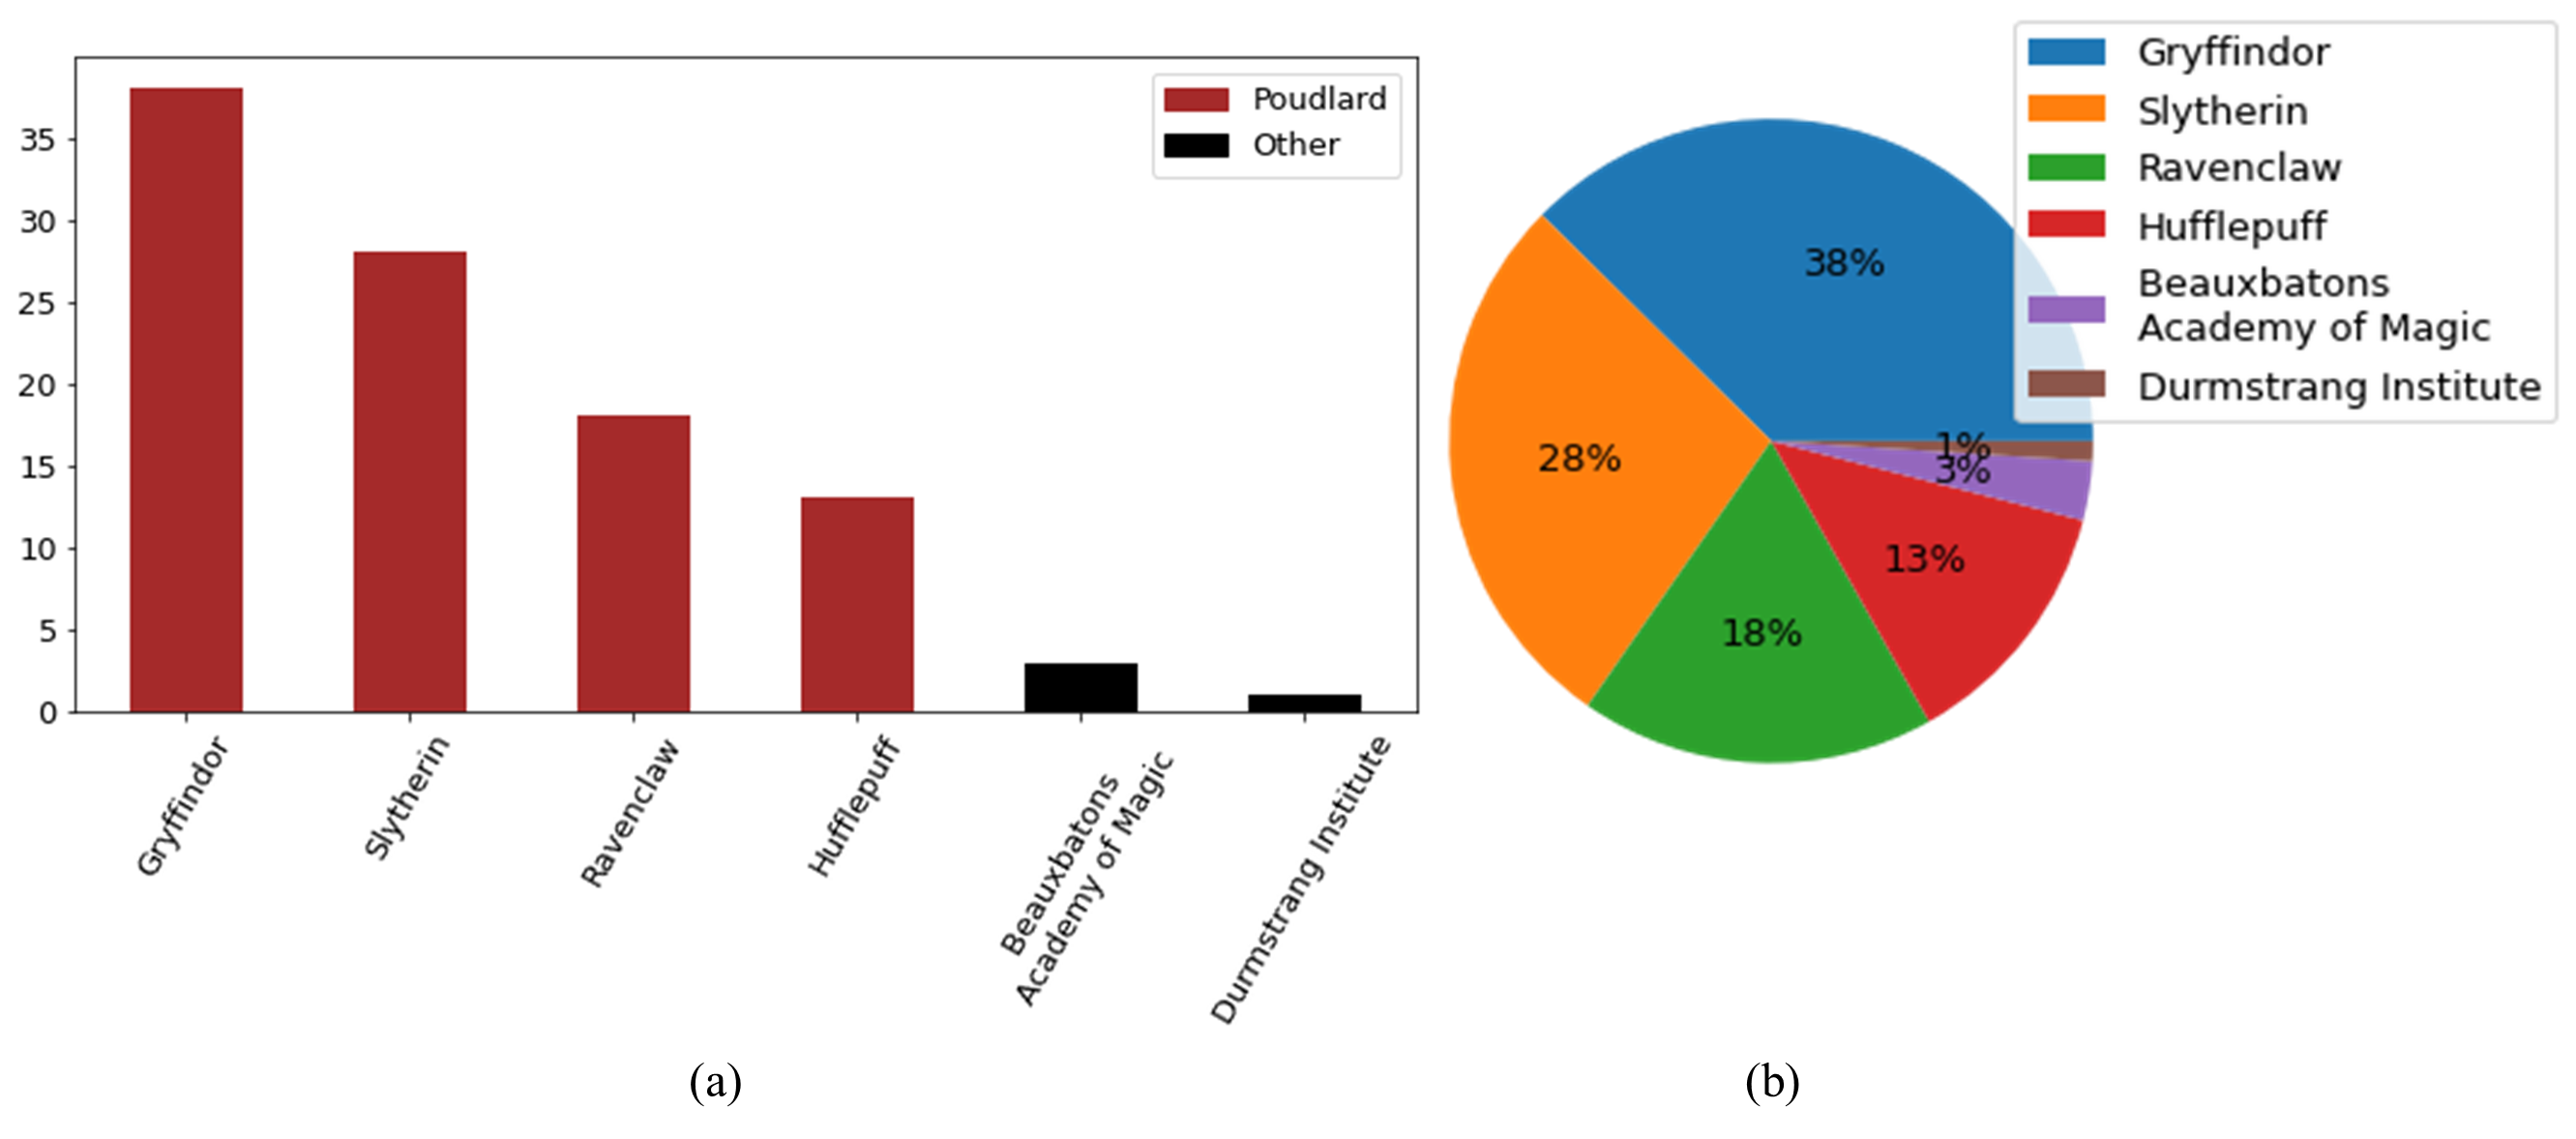
\includegraphics[width= 18 cm]{./figures/rep-houses.png}
    \caption{Regroupement des maisons et répartition des personnages par maison}
\end{figure}

La Figure 1.a représente la répartition des personnages selon les maisons. Nous remarquons que 66\% des personnages appartiennent aux maisons Gryffindor et Slytherin. En outre, nous constatons que le pourcentage des personnages des maisons "Beaubatons" et "Drumstrang" ne dépassent pas 4\%. Selon la Figure 1.b, ces dernières appartiennent à des écoles différentes de Poudlard.\par

Nous étudions dans la suite le lien entre les caractéristiques des personnages (principalement le sexe et le statut sanguin) et l'appartenance à une maison.\par

\begin{figure}[hbt!]
    \centering
    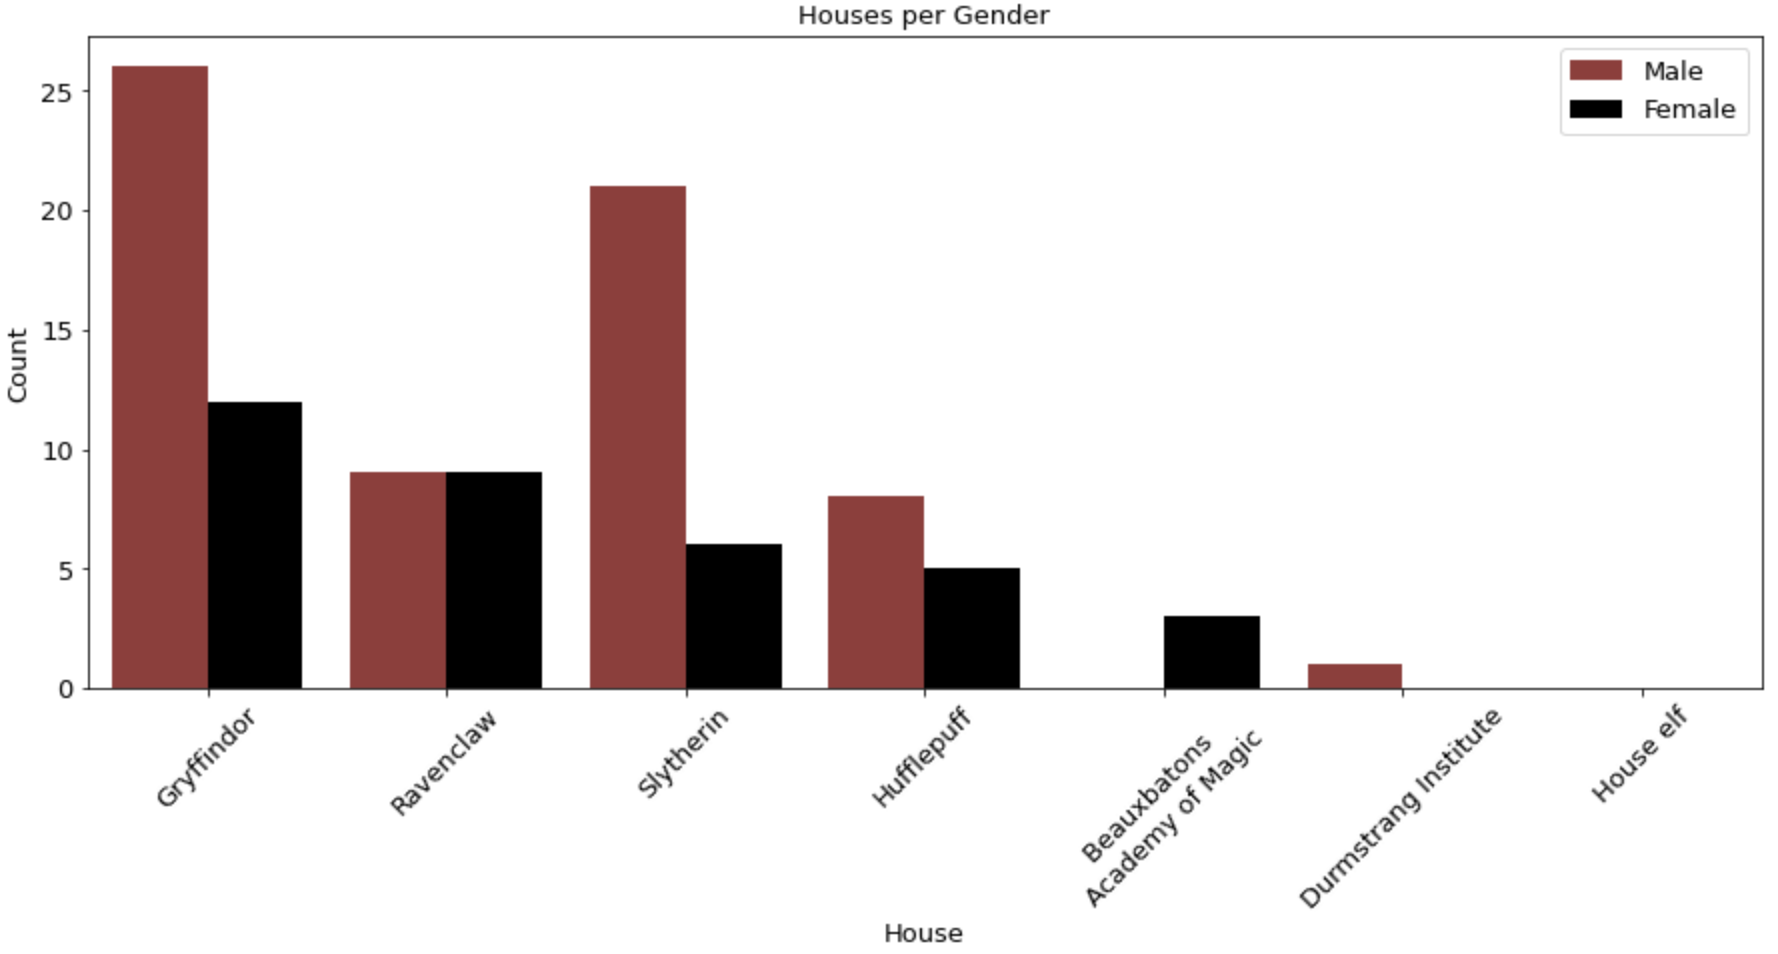
\includegraphics[width= 16 cm]{./figures/gender.png}
    \caption{Répartition des genres par maison}
\end{figure}
\FloatBarrier

La Figure 2 représente la répartition des personnages par sexe dans chaque maison. Nous remarquons que les maisons Poudlard contiennent des garçons et des filles, alors que les autres écoles sélectionnent selon le sexe.\par

La Figure 3 décrit les différents statuts sanguins présents dans chaque maison.

\begin{figure}[hbt!]
    \centering
    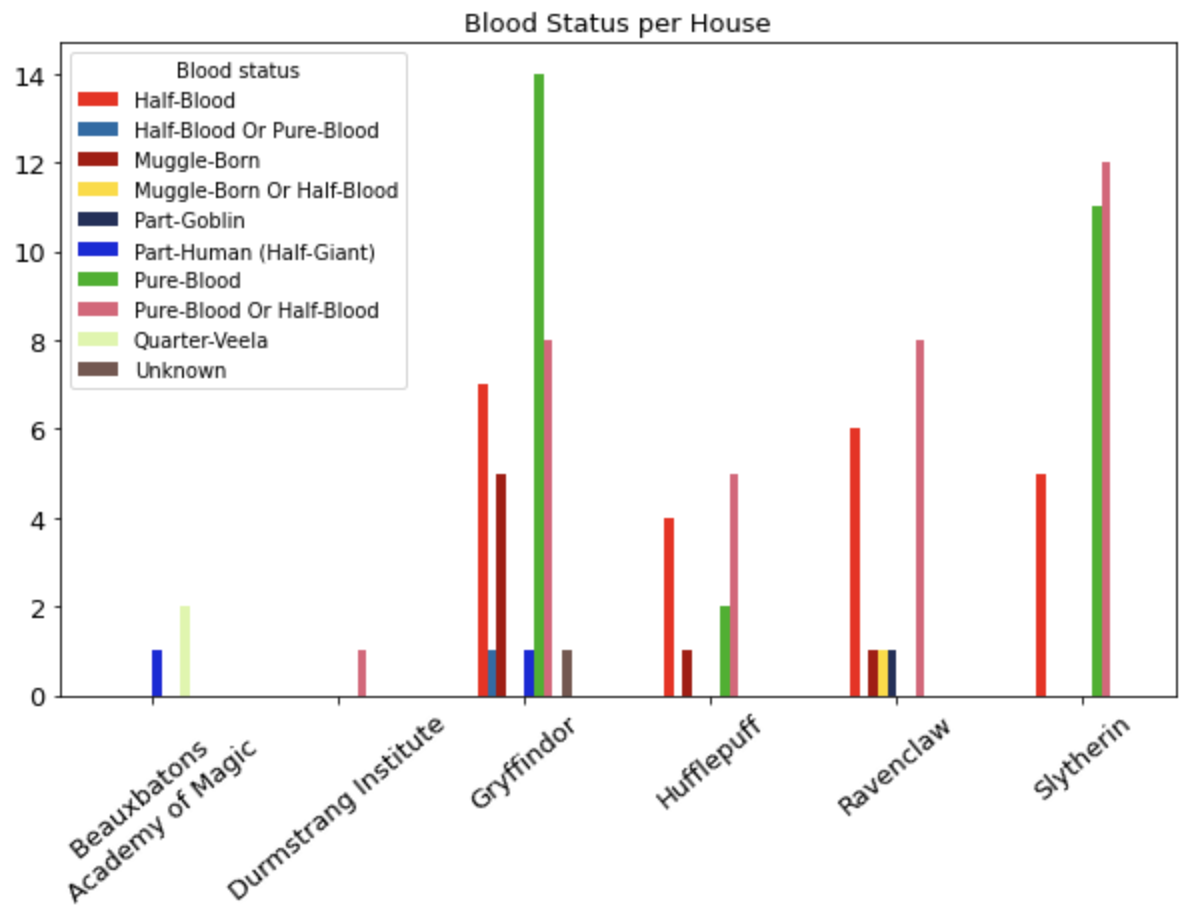
\includegraphics[width= 13cm, height= 8 cm]{./figures/blood_status.png}
    \caption{Repartition du statut de sang par maison}
\end{figure}
\FloatBarrier

Nous remarquons que les sang de type "Pure-Blood" et "Half-Blood" dominent toutes les maisons de l'école Poudlard. De plus, dans cette école, le type "Part-Human" caractérise une partie de personnages appartenant à la maison Gryffindor. La figure montre aussi que le type "Quarter-Veela" est absent de toutes les maisons sauf "Beauxbatons". Nous pouvons prévoir que le statut sanguin est une variable significative dans la classification des personnages.\par

Dans la suite, nous manipulons les données textuelles (les scripts) grâce à des méthodes de "text mining" pour savoir, dans la forme la plus courte possible, combien et que disent les personnages de ces 3 films, quel est le sentiment de leurs déclarations, quels mots ils utilisent souvent et bien plus encore.\par

Avant de "fouiller" dans le texte, nous commençons par regarder les nombres de phrase par personnage. La figure 4 représente les 15 premiers personnages qui parlent le plus.

\begin{figure}[hbt!]
    \centering
    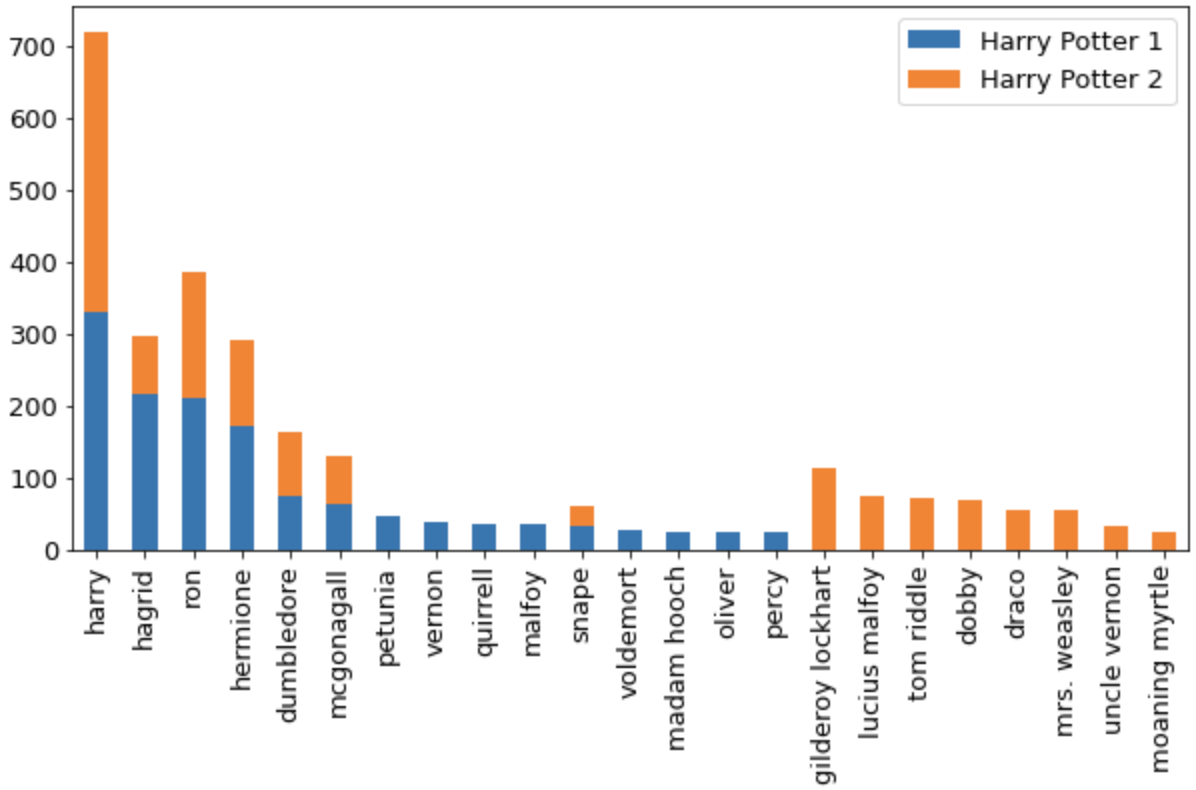
\includegraphics[width= 13cm, height= 8 cm]{./figures/most.png}
    \caption{Les personnages parlant le plus dans les 2 premiers films}
\end{figure}
\FloatBarrier

On remarque que la première place est occupée par le personnage principal Harry Potter, qui gagne avec 720 phrases. En deuxième place, on trouve Ron, l'ami de Harry. De plus, au premier plan, nous trouverons de nombreux professeurs de Poudlard, les amis de Harry et le méchant de toute la saga - Lord Voldemort. Certains personnages n'apparaissent que dans une partie et parviennent quand même à figurer parmi les personnages avec le plus grand nombre de dialogues. Un tel personnage est Gilderoy Lockhart, qui a prononcé plus de 100 discours dans la deuxième partie de la série de films.\par

Le "text mining" est l'art de transformer du texte libre en variables numériques, puis de les analyser avec des techniques statistiques. Afin d'appliquer cette analyse, nous avons effectué deux types de graphiques qui implémentent l'approche la plus courante du text mining : un wordcloud et des barplots de n-grammes.\par

La Figure 5 représente un wordcloud ( nuage de mots-clés) avec tous les mots mentionnés au moins 9 fois dans le script des deux premiers films.

\begin{figure}[hbt!]
    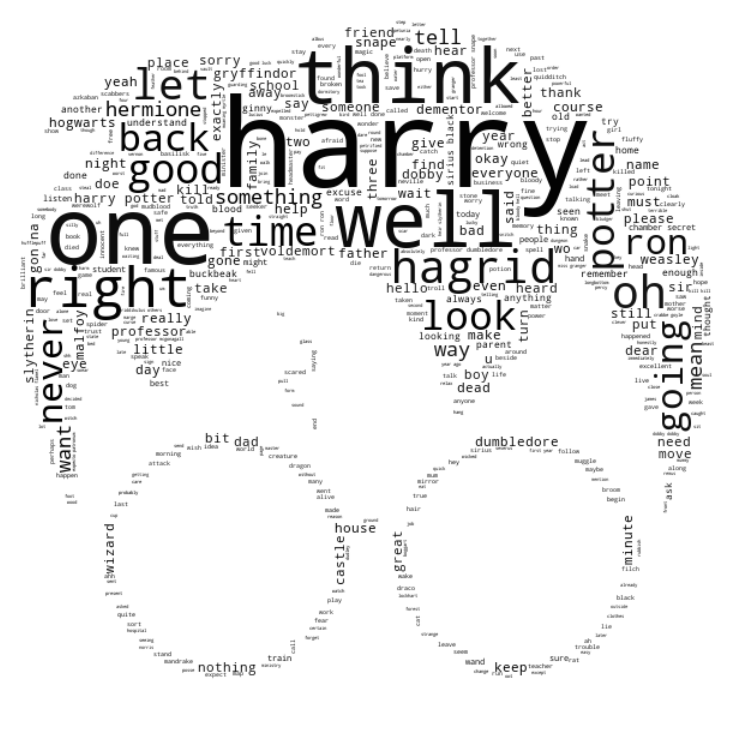
\includegraphics[width= 16cm]{./figures/wordcloud.png}
    \caption{Wordcloud des 2 premiers films}
\end{figure}
\FloatBarrier

Les mots s'affichent dans des tailles et graisses de caractères d'autant plus visibles qu'ils sont utilisés ou populaires. Nous remarquons donc que les trois mots les plus populaires sont "harry", "one" et "well".\par

Un n-gramme est une séquence contiguë de mots dans un texte. Nous commençons par étudier les bigrammes des deux premiers films.

\begin{figure}[hbt!]
    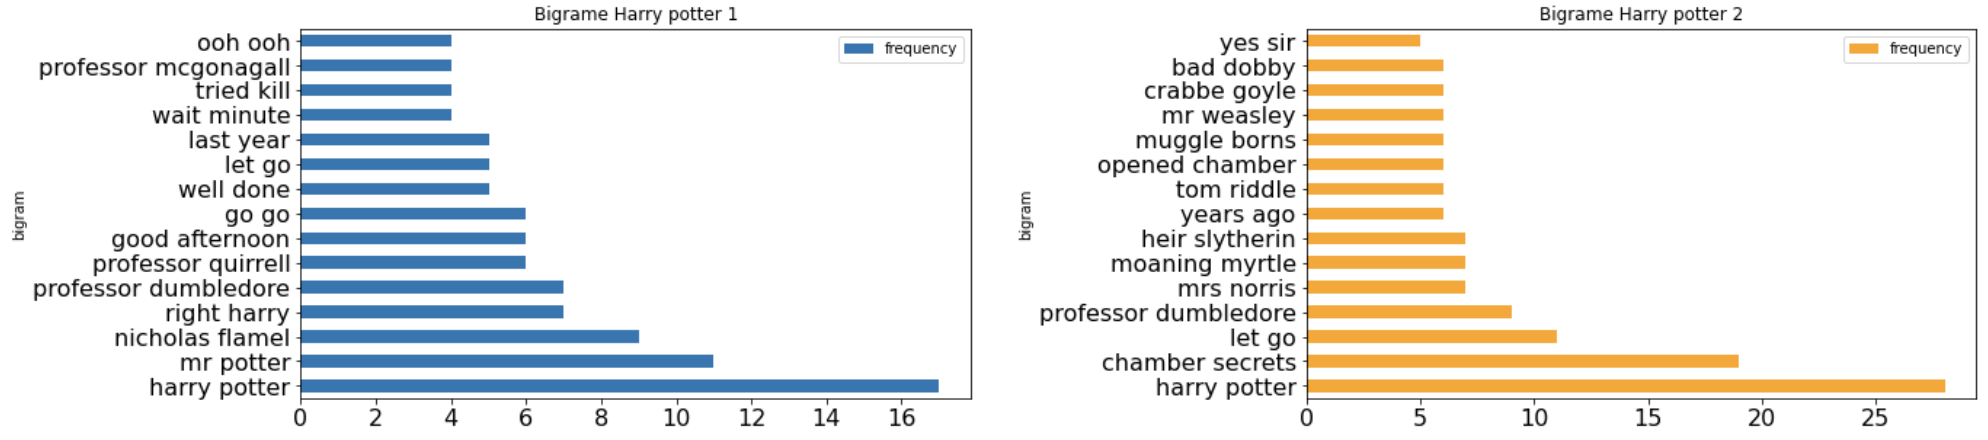
\includegraphics[width= 16cm, height= 7 cm]{./figures/bigrams.png}
    \caption{Top 15 bigrammes des 2 premiers films}
\end{figure}
\FloatBarrier

On remarque que le bigramme le plus populaire s'est avéré être "harry potter", qui est apparu dans les 2 premiers chapitres de la saga 47 fois au total. Parmi les personnages figurent également "nicholas flamel", "tom riddle", "professor dumbledore", "mrs morris", etc. La place suivante est occupée par des expressions courantes dans le discours de tous les jours telles que "good afternoon", "well done", ou encore "yes sir". Un bigramme dans le deuxième chapitre semble intéressant et unique : "heir slytherin".\par

La Figure 7 représente les 15 trigrammes les plus utilisés dans les chapitres 1 et 2.

\begin{figure}[hbt!]
    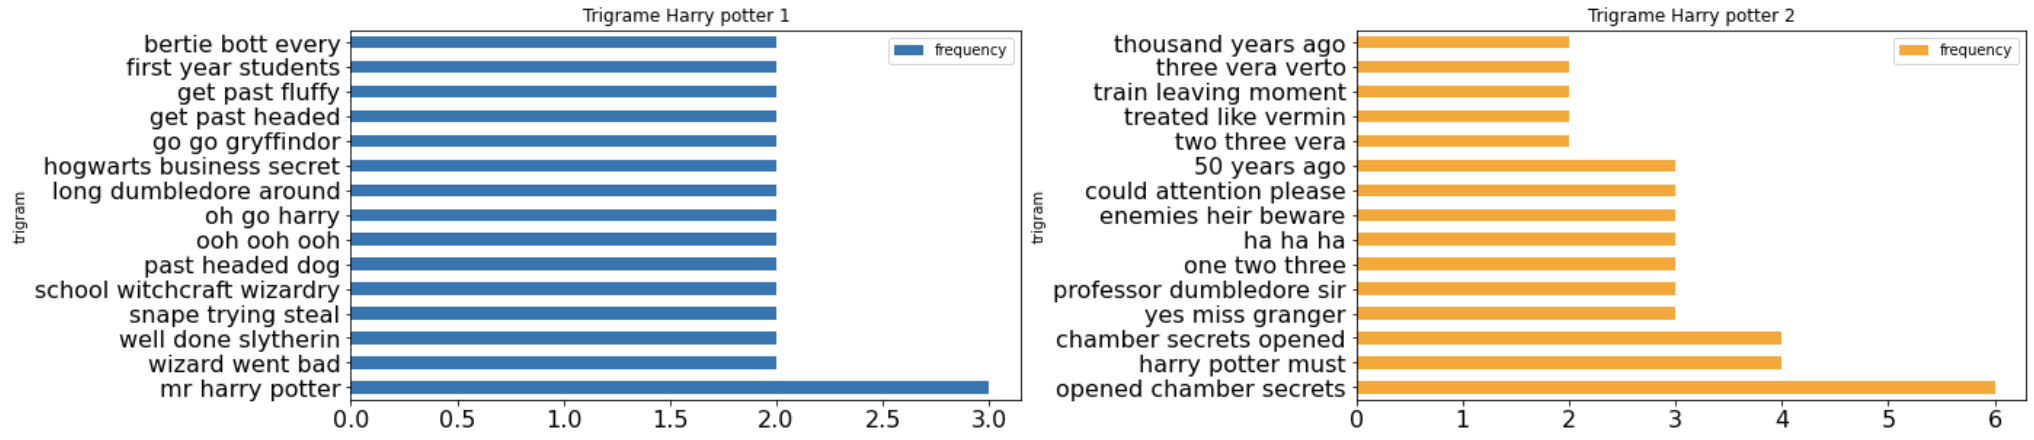
\includegraphics[width= 16cm, height= 7 cm]{./figures/trigrams.png}
    \caption{Top 15 trigrammes des 2 premiers films}
\end{figure}
\FloatBarrier

Nous remarquons que les trigrammes ont des fréquences plus petits car une séquence de 3 mots dans le même ordre est beaucoup moins courante qu'une séquence de 2 mots. Une partie du titre du deuxième film "opened chamber secrets" s'est avérée être le trigramme le plus populaire dans ce chapitre. Alors que, pour le premier film, le trigramme le plus populaire est "mr harry potter".Dans les trigrammes populaires, mis à part les phrases bien connues du discours quotidien, les éléments intéressants sont "hogwart business secret" et "school witchcraft wizardry", , que nous ne trouverons certainement pas dans le discours quotidien ou dans d'autres films.\par

L'analyse émotionnelle représente une des applications les plus utilisées dans le NLP. Dans cette optique, nous exploitons le traitement de texte effectué précédemment pour étudier le degré d'affect émotionnel dans le discours des personnages.\par

\begin{figure}[hbt!]
    \centering
    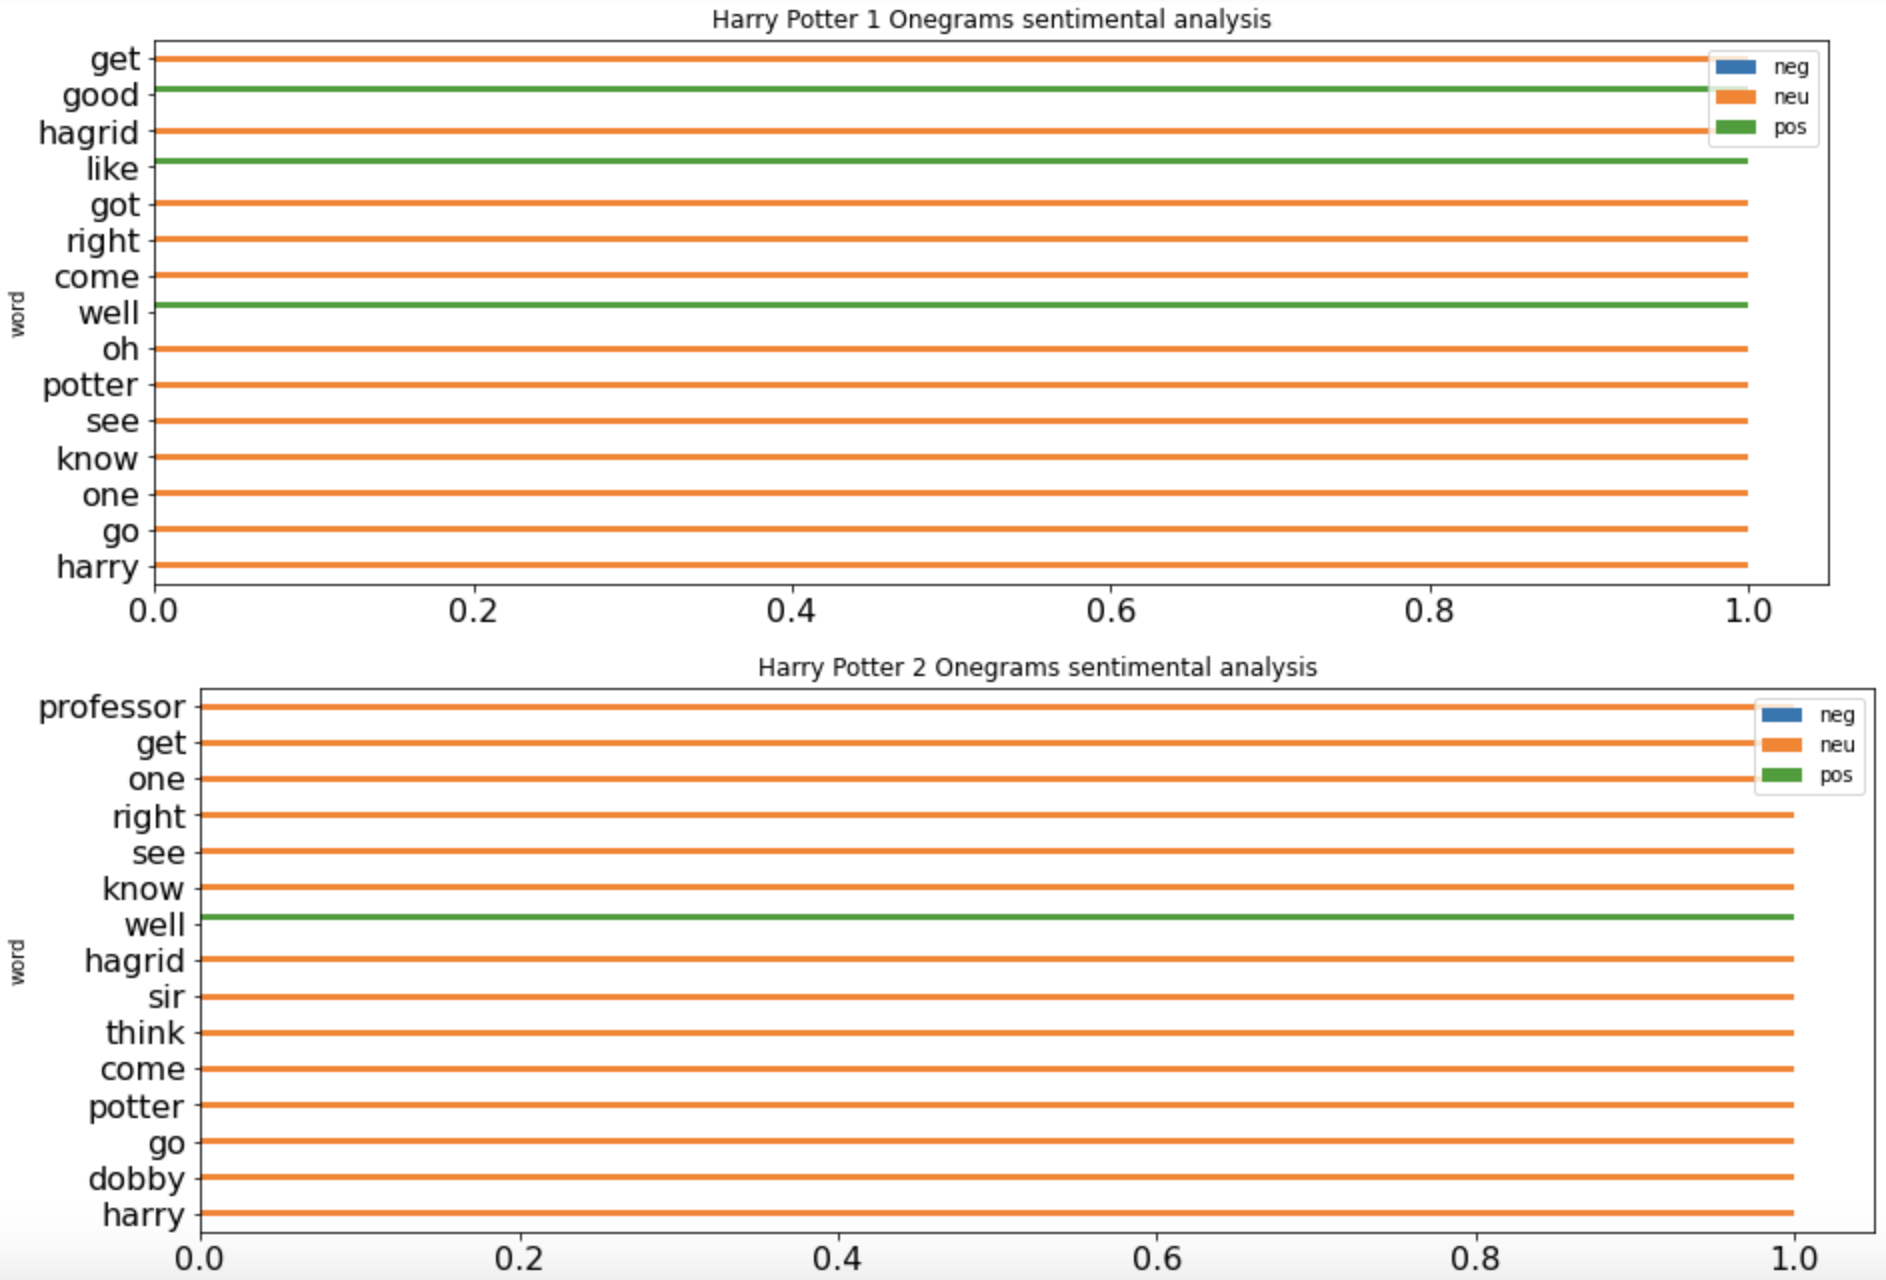
\includegraphics[width= 17 cm]{./figures/emotions_onegrams.png}
    \caption{Analyse des émotions par un-grammes}
\end{figure}
\FloatBarrier
\begin{figure}[hbt!]
    \centering
    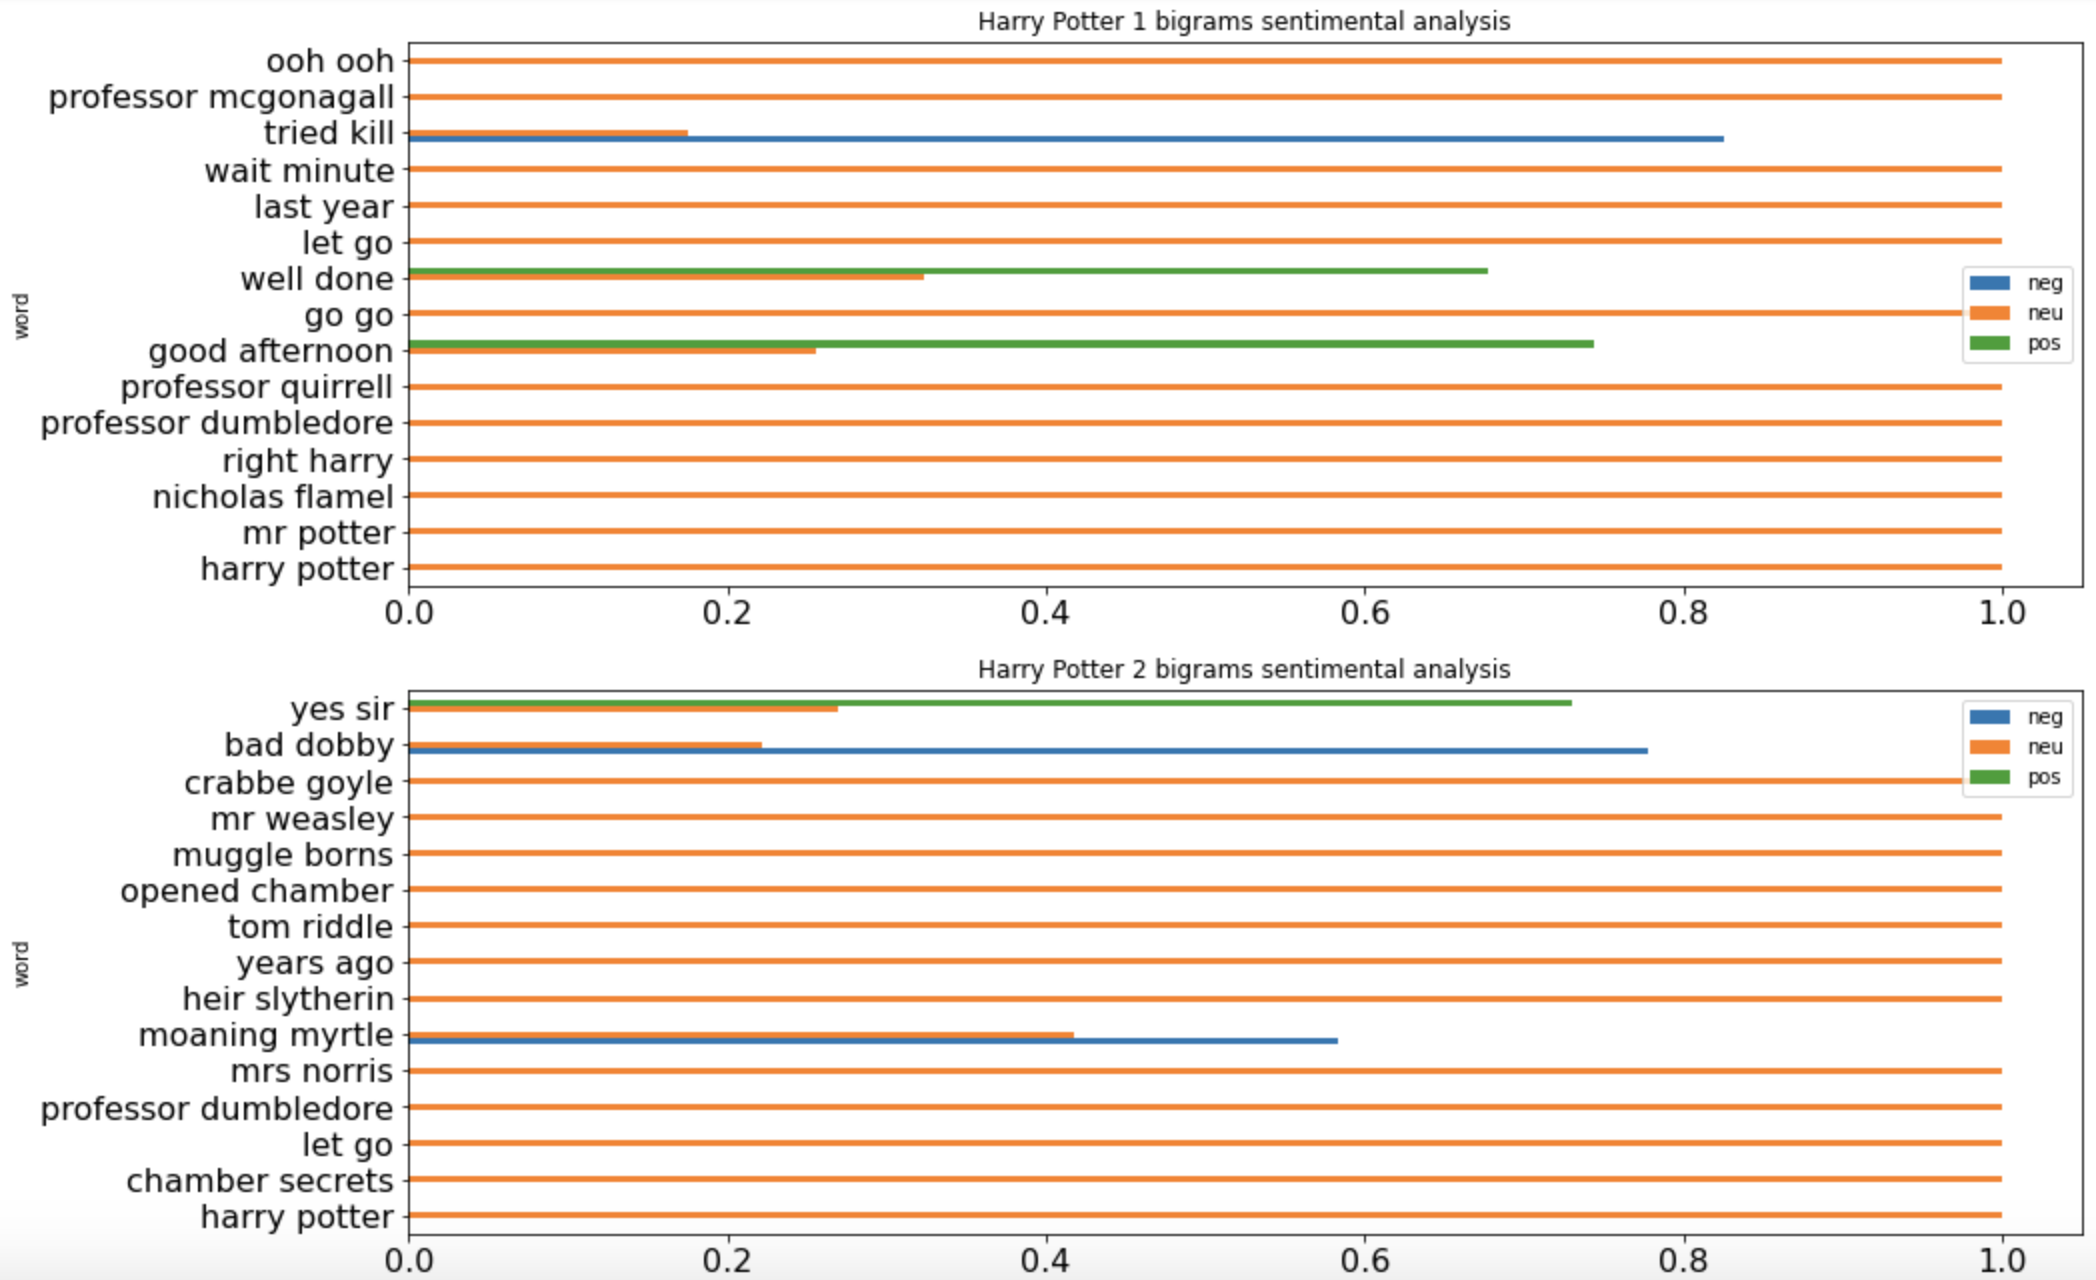
\includegraphics[width= 17 cm]{./figures/emotions_bigrams.png}
    \caption{Analyse des émotions par bigrammes}
\end{figure}
\FloatBarrier

NRCLeX est une bibliothèque Python qui contient un dictionnaire des affects avec environ 27 000 mots et qui se base sur le lexique des affects du Conseil National de Recherches du Canada (CNRC) et sur les ensembles des synonymes Wordnet de la bibliothèque NLTK. Dans le cadre de ce projet, nous utilisons cette bibliothèque pour générer les émotions à partir d'un corps de texte vue la difficulté de construire un modèle dédié à cette analyse. Les affects émotionnels mesurés par NRCLeX sont : la peur, la colère, l'anticipation, la confiance, la surprise, la positivité, la négativité, la tristesse, le dégoût et la joie.\par

La figure \autoref{emotions} représente les différentes émotions pour chaque maison mesurées à partir des personnages qui y appartiennent.

\begin{figure}[hbt!]
    \centering
    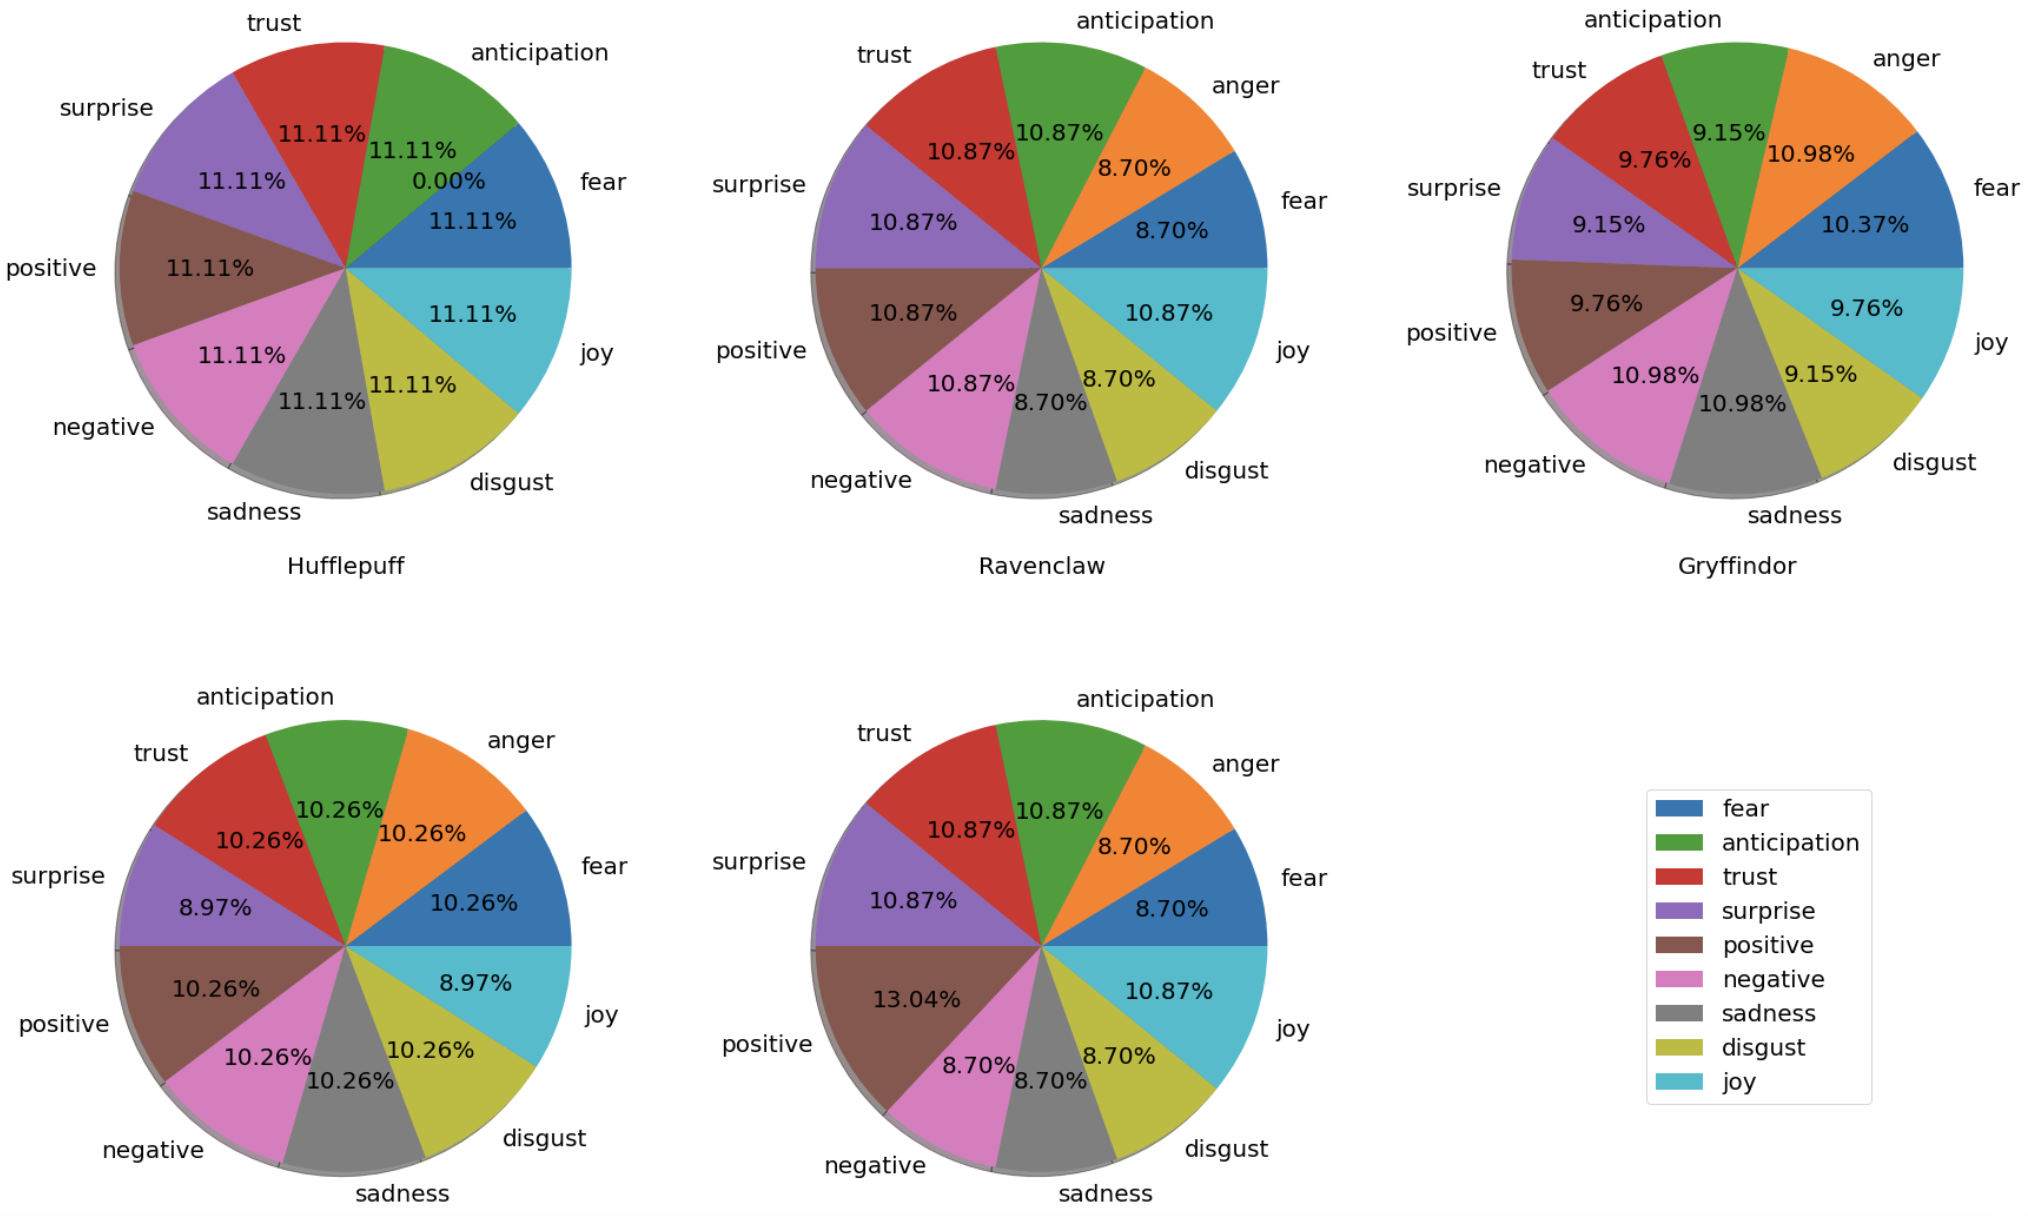
\includegraphics[width= 17 cm]{./figures/emotions_houses.png}
    \caption{Analyse des émotions par maison}
\end{figure}
\FloatBarrier

Nous remarquons que la colère est une émotion non-exprimée par les personnages de la maison "Hufflepuff". De plus, le comportement émotionnel général de la maison "Slytherin" s'oppose à celui de "Gryffindor"; principalement au niveau des émotions "positive", "négative", "sadness" et "anger". D'autre part, ce comportement est quasiment similaire à celui de la maison "Ravenclaw" sauf au niveau de la positivité et la négativité.\par

\begin{remarque}
    Nous utilisons les émotions exprimées par personnage comme variables explicatives dans la matrice de design.
\end{remarque}

%------------------------------------------------------%
\subsection{Matrice de design}
%------------------------------------------------------%

Cette partie est consacrée à la construction de la matrice {X} à laquelle seront appliquées les méthodes statistiques, appelée matrice de design. Chacune de ses lignes correspond à un individu statistique, ici les personnages, et ses colonnes contiennent les variables explicatives, que nous determinerons dans la suite, et la variable à expliquer {Y} étant les maisons de Poudlard.\par

\subsubsection{Variable à expliquer}

Etant donné que notre but est de prédire l'appartenance d'un nouveau personnage à une maison, pour ne pas des données qui nous serviront à alimenter les méthodes statistiques, nous choisissons d'inclure également les personnages n'appartenant à aucune des maisons de Poudlard sous la variable \textit{'Other'}. Ainsi nous obtenons cinq variables de "maison" ("Gryffindor", "Slytherin", "Ravenclaw", "Hufflepuff" et "Other") et pourrons inclure dans nos prédictions si un personnage apartient ou pas à une de maisons de Poudalard.\par

\subsubsection{Variables explicatives}

En plus des variables de genre et de statut de sang vues précedemment nous considérons les variables suivantes issues des scripts :

\begin{itemize}
    \renewcommand{\labelitemi}{$\bullet$}
    \item \textbf{Mots les plus communs :} En appliquant la fonction \textit{most\_common(10)} au script néttoyé, nous obtenons la liste des dix mots les plus prononcés et leur valeur correspondante : \\
    ('harry', 194), ('potter', 95), ('one', 86), ('well', 76), ('think', 75), ('hagrid', 74), ('right', 72), ('oh', 61), ('dobby', 60), ('would', 57).\\
    On remarque qu'en plus des noms de certains personnages, elle contient aussi des mots génériques ou encore une onomatopée, qui ne font partie de l'univers d'Harry Potter.\par
    Nous choisisons donc d'élargir la liste et de ne garder que dix mots liés à cet univers parmi les mots les plus dits : \\
    ('professor', 57), ('sir', 53), ('hogwarts', 38), ('slytherin', 38), ('school', 34), ('year', 33), ('gryffindor', 33), ('kill', 32), ('chamber', 32), ('wizard', 31).

    \item \textbf{Mots les plus communs :} Nous comptons le nombre de mots prononcés par chaque personnage et les ordonnons en fréquences.

\end{itemize}

Voici les premières lignes de la matrice de design obtenue pour les deux premiers opus de la saga :

\begin{figure}[hbt!]
    \centering
    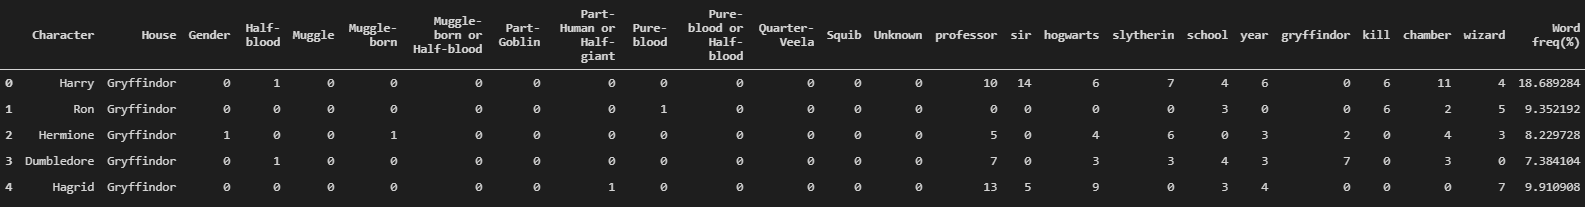
\includegraphics[width= 17 cm]{./figures/script_matrix.png}
    \caption{Matrice de design issue du script}
\end{figure}

\subsubsection{Variables additionnelles}

Nous pourrons par la suite, si les résultats statistiques le suggèrent, ajouter des caractérisques propres aux personnages, présentes dans les données "Characters.csv". En effet, les variables \textit{skills} et \textit{loyalty} pourront se révéler utiles quant à l'ajout d'information aux méthodes statistiques de classification.\par

%------------------------------------------------------%
%------------------------------------------------------%
\section{Analyse statistique}
%------------------------------------------------------%
%------------------------------------------------------%

Dans cette section, nous exploitons la matrice de design extraite de l'analyse de données afin de construire un modèle statistique capable de classifier des personnages dans les maisons de Poudlard. Dans cette optique, nous entraînons plusieurs modèles de classification pour choisir le plus adapté à notre cas d'étude en se basant sur les métriques de performance.\par

%------------------------------------------------------%
\subsection{Méthode des k plus proches voisins}
%------------------------------------------------------%

L’algorithme des K plus proches voisins ou K-nearest neighbors (k-NN) est un algorithme de Machine Learning qui appartient à la classe des algorithmes d’apprentissage supervisé.
\fb{conseil : couper les phrases un peu longue}
Cet algorithme  qui est simple et facile\fb{expliquer pourquoi c'est simple, même brievement} à mettre en œuvre peut être utilisé pour résoudre les problèmes de classification et de régression.{\cite{3}}\par

\subsubsection{Principe :}

\flo{Inverser les deux sous paragraphe. D'abord expliquer le principe. Ensuite dire qu'il n'y a pas de période d'apprentissage.}

Son principe est simple. Afin de déterminer la classe d'un individu n'appartenant pas au jeu de données, l'algorithme calcule la distance de celui-ci à tous les autres, collecte les classes des $k$ individus les plus proches et effectue un vote majoritaire dont la résultante sera la classe prédite pour le nouvel individu.\par
Cette méthode est souvent qualifiée de \textit{Lazy learner} provenant du fait qu'elle n'aie pas besoin de phase d'apprentissage.
En k-NN stocke l'ensemble des données et se repose dessus afin d'effectuer un prédiction.\par


\subsubsection{Notion de distance :}

Comme dit plus haut, le k-NN nécessite une fonction de calcul entre deux individus (observations) afin d'évaluer la notion de "similarité", plus la distance est petite, plus les individus sont similaires.
On note à ce titre, plusieurs distances peuvent être utilisées selon le type de données. Soient $n$ \fb{pensez à toujours mettre $n$, $p$ etc entre dollars} le nombre de variables et $(x,y) \in \mathbb{R}^{n} \times \mathbb{R}^{n}$ deux individus, voici deux exemples classiques de distance :
    \begin{itemize}
    \renewcommand{\labelitemii}{-}
        \item Distance euclidienne : $d_{e}(x,y)=\sqrt{\sum_{j=1}^{n}\left(x_{j}-y_{j}\right)^{2}}$

        \item Distance de Manhattan : $d_{m}(x,y)=\sum_{j=1}^{n}\left|x_{j}-y_{j}\right|$
    \end{itemize}
\fb{quelle distance allez-vous utiliser ?}
\fb{si vous parlez de 2 distances différentes, vous devez dire quand est-ce qu'une est préfèrable à uen autre }

\subsubsection{Algorithme :}
Récapitulons maintenant les étapes du k-NN :

    \begin{itemize}
        \item Entrées :
            \begin{itemize}
                \item Un jeu de données.
                \item Une distance d.
                \item Un nouvel individu $x \in \mathbf{R}^{n}$ à classifier.
                \item Un nombre entier k.
            \end{itemize}
            
        \item Traitement :(trouver un autre nom peut-être)Entraînement ?
            \begin{enumerate}
                \item Calcul des distance entre $x$ et tous les points du jeu de données.
                \item Détermination des k plus proches "voisins".
                \item Collecter les classes de ces k points.
                \item Attribuer la classe la plus présente à $x$.
            \end{enumerate}
        
        \item Sortie : classe prédite de $x$.
    \end{itemize}

Voici un exemple graphique pour illustrer cette méthode :

\begin{figure}[hbt!]
    \centering
    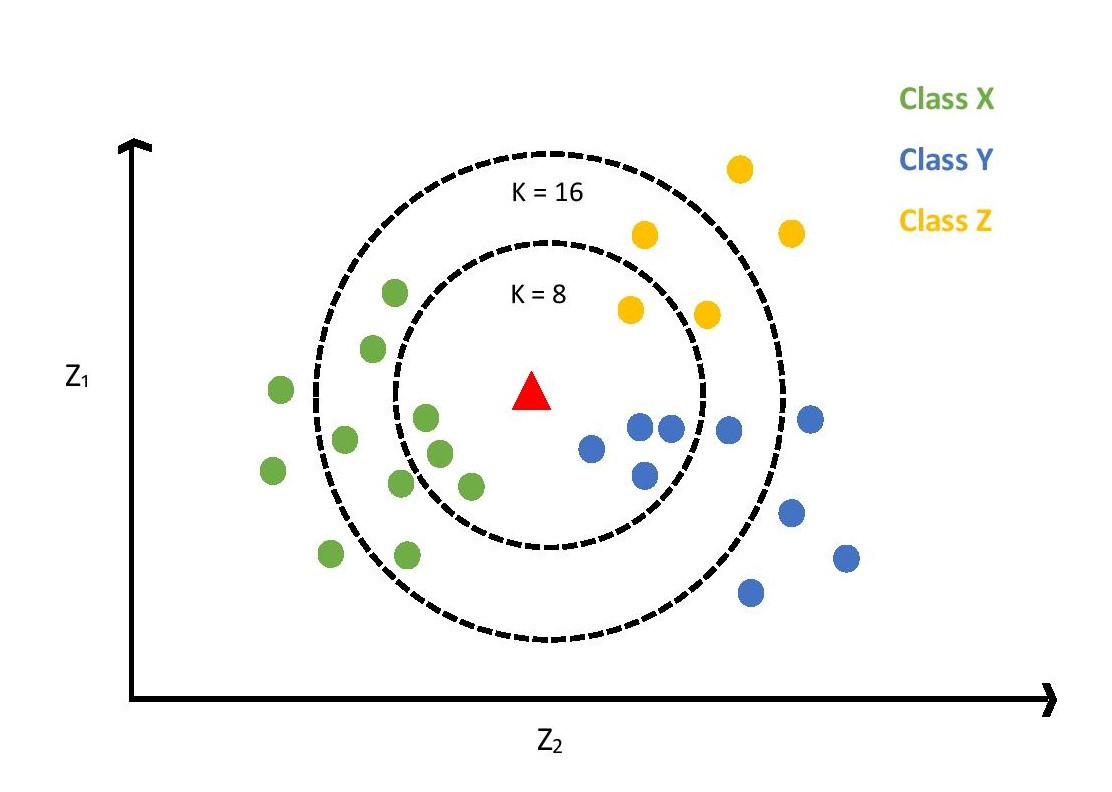
\includegraphics[width = 15 cm]{./figures/knn_example.jpeg}
    \caption{Exemple simple de l'algorithme k-NN (source: \cite{5}, auteur: Tharuka Sewwandi).}
    \label{12}
\end{figure}
\FloatBarrier

\subsubsection{Paramètres et implémentation}

\begin{itemize}
    \item \textbf{Le nombre de voisins k ("n\_neighbors") :}
    Sur la figure \ref{12} on remarque que selon la valeur de k, la classe du nouvel individu change. En effet, sur cet exemple si k=8 la classe attribuée est Y, alors que si k=16, le nouveau point appartient à la classe X. Ceci illustre bien l'importance du choix du paramètre k.\par
    
    \item \textbf{La fonction de distance ("metric") :}
    Comme dit plus haut, le k-NN nécessite une fonction de calcul entre deux individus (observations) afin d'évaluer la notion de "similarité", plus la distance est petite, plus les individus sont similaires.
    On note à ce titre, plusieurs distances peuvent être utilisées selon le type de données. Soient n \fb{pensez à toujours mettre $n$, $p$ etc entre dollars}le nombre de variables et $(x,y) \in \mathbf{R}^{n}$x$\mathbf{R}^{n}$ deux individus, voici deux exemples classiques de distance :
        \begin{itemize}
        \renewcommand{\labelitemii}{-}
            \item Distance euclidienne : $d_{e}(x,y)=\sqrt{\sum_{j=1}^{n}\left(x_{j}-y_{j}\right)^{2}}$
        
            \item Distance de Manhattan : $d_{m}(x,y)=\sum_{j=1}^{n}\left|x_{j}-y_{j}\right|$
        \end{itemize}
        
    \item \textbf{Le poids des individus ("weights") :}
    L'algorithme k-NN propose d'affecter ou pas des poids aux individus en fonction de leur distance au nouveau point.
        \begin{itemize}
        \renewcommand{\labelitemii}{-}
            \item "uniform" : l'ensemble des individus du jeu de données ont un même poids.
            
            \item "distance" : plus un individu est proche/similaire (au sens de la métrique) du nouveau point, plus son poids est grand.
        \end{itemize}
\fb{quelle distance allez-vous utiliser ?}
\fb{si vous parlez de 2 distances différentes, vous devez dire quand est-ce qu'une est préfèrable à uen autre }
\end{itemize}

Une méthode de détermination de ces paramètres est d'essayer toutes les combinaisons possibles et comparer les scores. Ces calculs sont automatisés sur Python grâce à la fonction GridSearchCV. 

Avant d'effectuer une validation croisée de notre modèle, nous prenons le soin de vérifier la stratification des classes. En effet nous remarquons que nos classes ne sont pas également réparties : 

    \begin{itemize}
        \item "Gryffindors" : 34
        \item "Slytherins" : 26
        \item "Ravenclaws" : 17
        \item "Hufflepuffs" : 13
        \item "Others" : 42,
    \end{itemize}

ce qui éviterait que le modèle sur-apprend certaines classes et en sous-apprend d'autres.\par
Voici la combinaison ayant obtenu la meilleure précision :

\begin{figure}[hbt!]
    \centering
    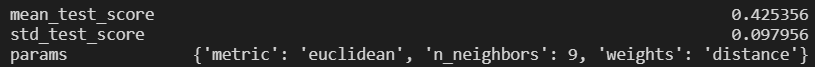
\includegraphics[width = 14 cm]{./figures/kNN_CV.png}
    \caption{Résultats de la validation croisée des paramètres de k-NN.}
    \label{kNN_CV}
\end{figure}
\FloatBarrier



\subsubsection{Comment choisir k ?}

Prendre en compte les remarques et supprimer cette partie

Sur la figure \autoref{12} on remarque que selon la valeur de k, la classe du nouvel individu change. En effet, sur cet exemple si k=8 la classe attribuée est Y, alors que si k=16, le nouveau point appartient à la classe X. Ceci illustre bien l'importance du choix du paramètre k.\par
Une méthode de détermination de k est de le faire varier et comparer les performances des modèles \flo{sur des données de tests}.(ou par validation croisée avec GridSearchCV)\par

\flo{On cherche toujours l'hyperparamètre avec une procédure de validation croisée, sinon, on fait forcement du surapprentissage et vous allez forcement selectionner le plus grand $k$. }

\flo{Vous y etes presque sur cette partie}
A TERMINER EN AJOUTANT UN GRAPHE ET LE CHOIX DE K

\subsubsection{Résultats}

%------------------------------------------------------%
\subsection{Forêts Aléatoires (Random Forests)}
%------------------------------------------------------%
\fb{Vous devez définir un minimum les arbres avant de définir les fôrets : au moins les grandes idées avec des mots !}

\subsubsection{Arbres de décision}

Le modèle \textbf{"Arbre de décision"} représente une pierre angulaire des forêts aléatoires. Ce modèle structure les données sous la forme d'un arbre.Il est construit de deux types d'éléments: les \textbf{nœuds} et les \textbf{branches}. À chaque nœud, une caractéristique (variable explicative) est évaluée pour prendre une décision de séparation, comme montre la Figure \ref{tree}:

\begin{figure}[hbt!]
    \centering
    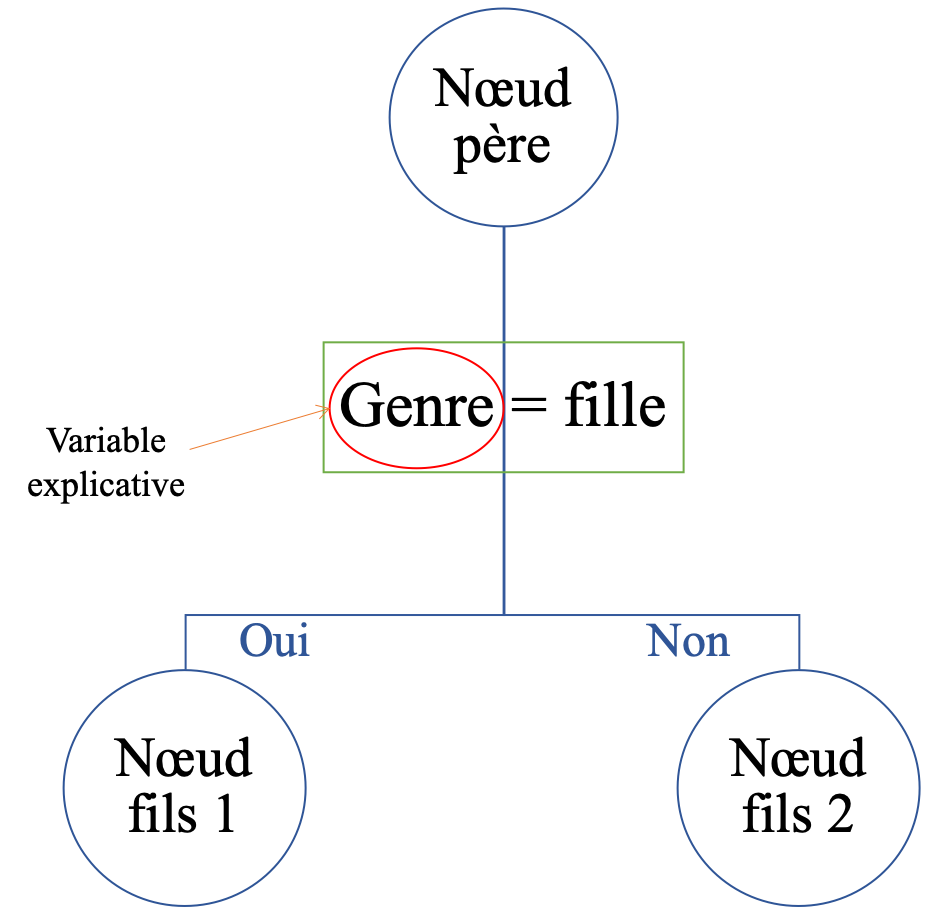
\includegraphics[width = 7 cm]{./figures/tree.png}
    \caption{Exemple simple d'arbre de décision}
    \label{tree}
\end{figure}
\FloatBarrier

Malgré les avantages fournis par le modèle d'arbre de décision tels que la simplicité, la transparence et l’interprétabilité des prédictions, ce modèle envisage des difficultés de stabilité à titre d'exemple la génération d'un nouvel arbre à chaque petite modification des données d’entraînement \cite{hands} et de sur-apprentissage dans le cas de la création d'un arbre complexe pour des données simple \cite{hands}.\par

Afin de surmonter ces difficultés, le modèle de \textbf{forêt aléatoire} permet d'avoir une prédiction plus précise et plus stable grâce à l’agrégation des prédictions provenant d'un ensemble d'arbres de décision.\par 

\subsubsection{Principe :}

Le modèle Random Forest \citep{breiman2001random}, abrégé RF, se base sur la méthode du \textbf{Bagging} (pour \textbf{Bootsrap Aggregating}).
Cette méthode consiste à échantillonner de manière aléatoire des sous-ensembles de données d'entraînement.
Ces données sont utilisées pour entraîner un nombre défini d'arbres de décision.
Une fois que tous ces prédicteurs sont formés, l'ensemble peut faire une prédiction pour une nouvelle instance en utilisant le \textbf{vote majoritaire} comme méthode d’agrégation de tous les prédicteurs.
Ce processus est décrit dans la Figure \autoref{RF}.\par

\flo{Attention, vous avez écrit Bagging sur votre graphique. C'est faux. Cette étape est celle de boostrap. Le bagging. C'est l'ensemble de la procédure.}

\flo{ATTENTION, l'algorithme random forest est basé sur le Bagging : Oui MAIS pour prendre en compte la correlation du à la construction des échantillons Boostrap, une étape a été ajouté : lorsqu'un cherche la meilleure variable à un noeud d'un arbre, on cherche seulement un sous-échantillon des variables et non l'ensemble des variables. C'EST IMPORTANT}
\begin{figure}[hbt!]
    \centering
    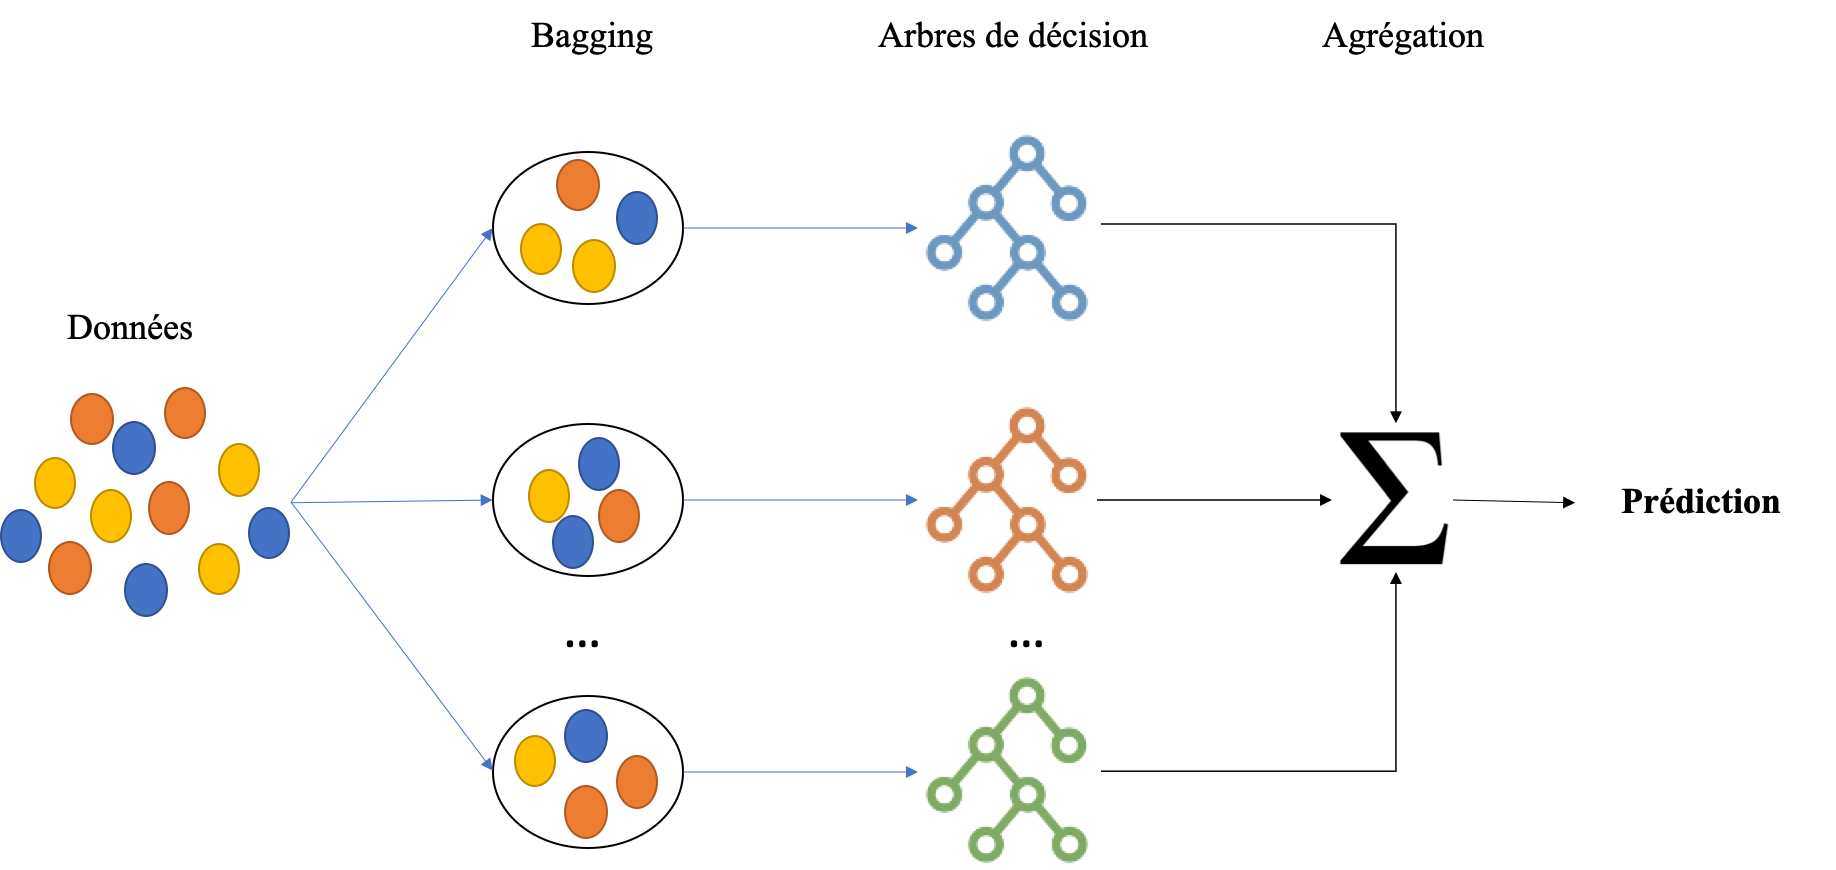
\includegraphics[width = 15 cm]{./figures/RF.png}
    \caption{Processus Random Forest}
    \label{RF}
\end{figure}
\FloatBarrier

\subsubsection{Algorithme :}

Récapitulons maintenant les étapes du RF :

    \begin{itemize}
        \item Entrées :
            \begin{itemize}
                \item Un jeu de données.
                \item Un nombre  N d’arbres de décision.
            \end{itemize}

        \item Entraînement :
            \begin{enumerate}
                \item Créer N échantillons du jeu de données .
                \item Créer N arbres de décision, et les entraîner chacun d'eux sur un échantillon différent.
                \item Effectuer une inférence en agrégeant les prédictions des arbres.
            \end{enumerate}

        \item Sortie : classe prédite de $x$.
    \end{itemize}

\fb{du coup, ceci est simplement du bagging d'arbres ! Pas random forest.}
\subsubsection{Paramètres et implémentation :}

Dans le cadre de notre étude, nous utilisons l'objet RandomForestClassifier de la bibliothèque \texttt{scikit-learn} \citep{scikit_learn}. Ses paramètres les plus importants sont :
\begin{itemize}
    \item \textbf{max\_features :} correspond aux nombres de features/attributs à chaque découpage d'arbre. \fb{option ? si max\_feautres est le nombre de variable, est-ce toujours l'algorithme des forêts aléatoires ou simplement du bagging.}
    \item \textbf{n\_estimators :} correspond aux nombres d'arbres. C'est un paramètre de type entier. Il est égale à 100 par défaut.
    \item \textbf{max\_depth :} le nombre maximal de niveau d'arbre de décision.
    \item \textbf{criterion :} fonction permettant de mesurer la qualité du découpage d'arbre.
    \flo{quelques paramètres utiles dans notre cadre : surtout : lass\_weight, max\_samples,potentiellement : min\_samples\_split,
    min\_samples\_leaf}
\end{itemize}

Le choix de ces paramètres varie selon la matrice de design. \fb{varie selon les données, problème, c'est plus général que seulement la matrice de design mais c'est l'idée}
Pour cela, nous faisons appel à une technique d'optimisation de paramètres appelé \textbf{hyperparameter tunning}.
\flo{pas très clair : chercher les hyperparamètres est un problème d'optimisation. Une façon de répondre à ce problème est de chercher toutes les combinaisons de paramètres possibles. C'est ce que fait GridSearchCV. Si il y a trop de combinaison, on fait une RandomGridSearchCV}
Cette technique est également implémentée au niveau de \texttt{sk-learn} en utilisant la classe \textbf{GridSearchCV} du modèle selection.
Elle va nous permettre d'automatiser la recherche d'un optimum parmi les hyperparamètres décrit dans la Figure \autoref{paramtunRF} en choisissant une validation croisée de dix blocs \fb{on utilise parfois folds même en français}.\par
\fb{globalement l'idée est la}

\begin{figure}[hbt!]
    \centering
    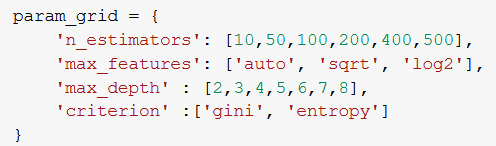
\includegraphics[width= 11 cm]{figures/paramtunRF.jpeg}
    \caption{Paramètres à optimiser}
    \label{paramtunRF}
\end{figure}
\FloatBarrier

Nous appliquons GridSearchCV sur les variables extraites purement des données textuelles en les répartissant 80\% pour l’entraînement et 20\% pour le test. Nous obtenons les paramètres suivants :

\begin{figure}[hbt!]
    \centering
    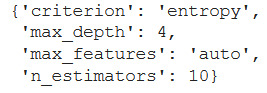
\includegraphics[width = 7 cm]{./figures/outputCVRF.jpeg}
    \caption{Hyperparamètres optimals}
    \label{CV1}
\end{figure}
\FloatBarrier

Nous entraînons notre modèle en se basant sur ces derniers résultats. Nous obtenons une précision sur les données du test d'environ 27\%.

La matrice de confusion est un outils résumant les résultats de prédictions. Les prédictions correctes et incorrectes sont mises en lumière et réparties par classe. Les résultats sont ainsi comparés avec les valeurs réelles.

\begin{figure}[hbt!]
    \centering
    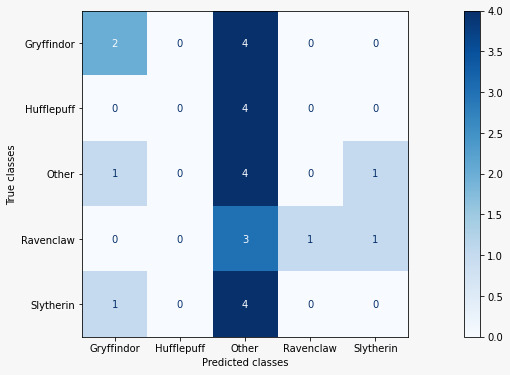
\includegraphics[width= 11 cm]{figures/matriceconfRF.jpeg}
    \caption{Matrice de confusion RF}
    \label{confRF}
\end{figure}
\FloatBarrier

La diagonale représente les bonnes prédictions. Nous remarquons donc que  le modèle a bien prédit la classe "Other". En revanche, il n'arrive pas à bien distinguer les autres classes; 57\% des personnages qui appartiennent à d'autres classes sont prédits comme "Other".\par

Afin d’améliorer notre modèle, nous avons ajouté aux données textuelles des variables caractéristiques qui décrivent chaque personnage. Nous ré-entraînons le modèle de la façon que le premier modèle et nous obtenons les résultats suivants:

\begin{figure}[hbt!]
    \centering
    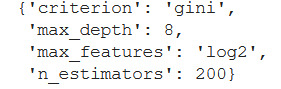
\includegraphics[width= 7 cm]{figures/outputCVRF2.jpeg}
    \caption{Hyperparamètres optimaux}
    \label{CV2}
\end{figure}
\FloatBarrier

Après l’entraînement d'un nouveau modèle en utilisant les paramètres de la Figure \autoref{CV2}, nous remarquons que sa précision est passée de 27\% à environ 57,7\%, ce qui signifie que les variables liées aux personnages ont pu aider le modèle à mieux distinguer les différentes classes.

\begin{figure}[hbt!]
    \centering
    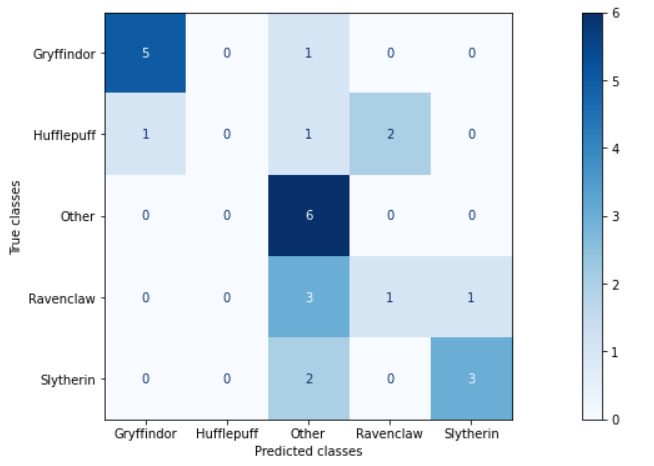
\includegraphics[width = 11 cm]{figures/matriceconfRF2.jpeg}
    \caption{Matrice de confusion RF}
    \label{confRF2}
\end{figure}
\FloatBarrier
La matrice de confusion (Figure \autoref{confRF2}) valide les performances du modèles. Nous remarquons une augmentation au niveau des prédictions correctes et une diminution des fausses prédictions.
De plus, le modèle n'a pas pu encore distinguer la maison "Hufflepuff", ce qui signifie que le modèle a besoin d'autres variables explicatives.\par


%------------------------------------------------------%
%------------------------------------------------------%
\section{Analyse statistique}
%------------------------------------------------------%
%------------------------------------------------------%

\flo{\textbf{Remarques générales:}
    \begin{itemize}
        \item Commencer par les K plus proches voisins.
        \begin{itemize}
            \item Definissez les K-plus proches voisins.
            Le modèle est simple et a un unique paramètre, le modèle est donc plus à optimiser.
            \item Le vote majoritaire peut ainsi être définis
            \item Ensuite, on peut dire qu'une autre façon de faire un vote majoritaire, c'est d'utiliser des méthodes d'aggregations, comme par exemple avec les arbres de décisions.
        \end{itemize}
        \item Il est \textbf{obligatoire} de définir ce qu'est un arbre avant de définir les forêts aléatoires, le bagging ou autre.
        \item Attention à votre orthographe.
        \item Soyez consistant dans vos notations !
    \end{itemize}
    }

%------------------------------------------------------%
\subsection{Estimateurs de variance élevée}
%------------------------------------------------------%

\flo{Définisser ce qu'est un arbre :
    \begin{itemize}
        \item  Quelle est l'idée simple derrière un arbre ?
        \item Representation graphique de l'idée en 2D (voir slide de Joseph)
        \item Discussion autour des avantages et inconvénients : ce que vous avez écrit dans la partie estimateur de variances élevés
    \end{itemize}
    }




Dans cette section nous examinons plusieurs stratégies pour construire (ou assembler) des classifieurs performants à partir de \flod{classifieurs de base plus modestes}.
\flo{Plus modeste n'a aucune définition statistique ! On a des critères objectifs permettant de dire quels sont les points forts et les points faibles d'un modèle}
On parle de « méthodes d’agrégation ». \fb{Dire en quoi cela consiste ?}
Nous allons commencer par une discussion des avantages et des défauts des arbres de décision\flod{, surtout le problème des estimateurs de variance élevée.}
\flo{Ce doit être fait dans la partie des arbres de décisions et vous devez expliquez pourquoi, par construction, les arbres ont une large variance et sont sensible aux variations dans le jeu de données !}
\fb{Pour le moment, on va se concentrer sur le bagging pour faire echo au KNN !}
Ensuite nous présenterons les deux approches classiques conçues pour répondre à ce problème : le « Bagging » et les « Forêts aléatoires » et nous finirons par expliquer le Boosting, qui permet de combiner la sortie de plusieurs classifieurs simples pour en obtenir un meilleur résultat.\par

%------------------------------------------------------%
\subsection{Estimateurs de variance élevée}
%------------------------------------------------------%

\begin{figure}[h!]
    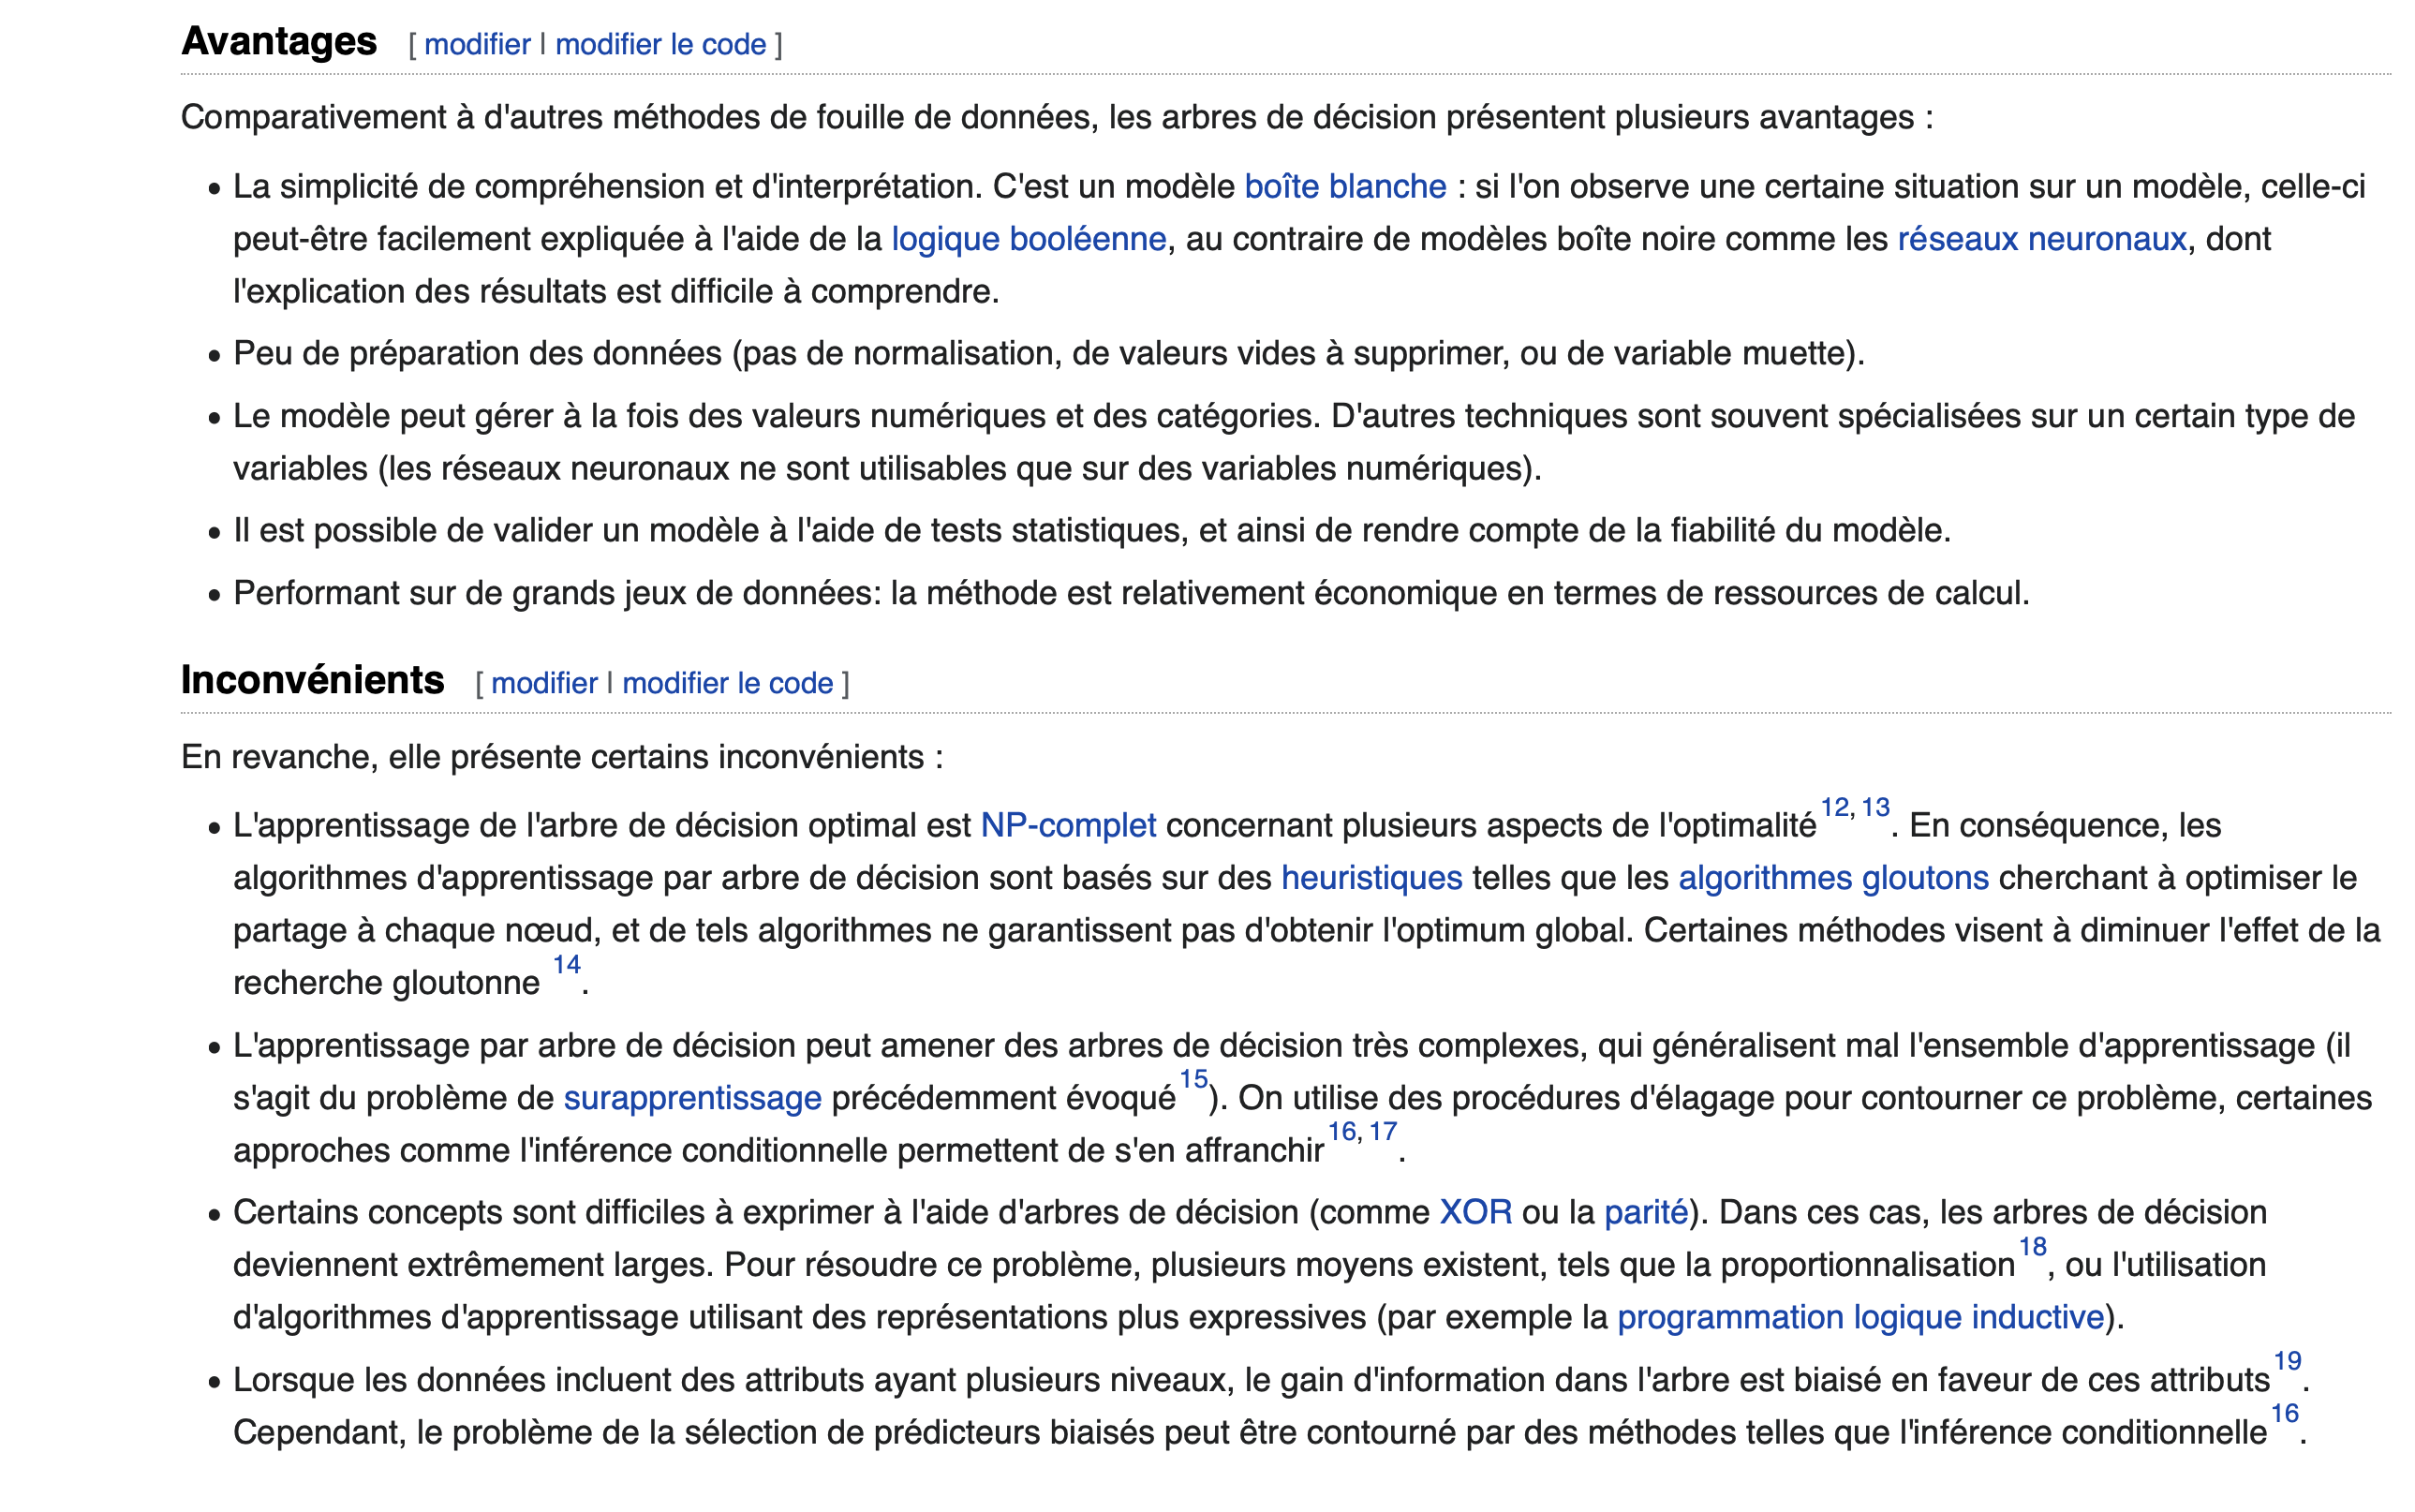
\includegraphics{figures/plagiat.png}
    \caption{Doit-on vous rappelez que le plagiat est interdit ?}
\end{figure}

\begin{itemize}
\renewcommand{\labelitemi}{$\bullet$}
\item \textbf{Avantages :}

    \begin{itemize}
    \renewcommand{\labelitemii}{-}
    \item La simplicité de compréhension et d'interprétation.
    \flo{Oui mais expliquer pourquoi et ATTENTION, c'est uniquement le cas pour \textbf{un unique} arbre de décision, on perd ces avantages dès qu'on fait une règle majoritaire}

    \item C'est un modèle boîte blanche\fb{terme flou} : si l'on observe une certaine situation sur un modèle \fb{qu'entendez vous par modèle ici ?}, celle-ci peut-être facilement expliquée à l'aide de la logique booléenne.
    Ce qui n'est pas le cas des boîtes noires comme les réseaux neuronaux, dont l'explication des résultats est difficile à comprendre.

    \item La méthode nécessite peu de préparation des données (pas de normalisation, de valeurs vides à supprimer, ou de variable muette). \flo{Vous ne pouvez pas dire ca sans comparer à d'autres méthodes pour lesquels c'est necessaire}
    \flo{Attention, la normalisation et la standardisation sont 2 choses (légèrement) différentes}
    \flo{Attention, normaliser ou standariser n'est pas toujours obligatoire, les KNN, la regression logistiques etc peuvent 'fonctionner' sans, mais c'est toujours mieux de normaliser/standardiser nos données}

    \item Il est possible de valider un modèle à l'aide de tests statistiques, et ainsi de rendre compte de la fiabilité du modèle.
    \flo{Vous ne pouvez pas dire cela sans donner de référence ou d'exemple}

    \item Performance \fb{préciser en termes computationnels ! C'est le cas pour l'estimation ? la prédiction ? les deux ?} sur de grands jeux de données: la méthode est relativement économique en termes de ressources de calcul.

    \item Ils sont capables de gérer des problèmes multi-classes. \\
    \flo{Techniquement, si un modèle ne gère que 2 labels mais que vous en avez 3, vous faites le label le plus nombreux contre les 2 autres dans un premier temps et ensuite les 2 plus petits dans un deuxième temps.}

    \end{itemize}

\flo{Si c'est utile, sa place n'est pas dans les annexes !}
(à mettre dans annexe quelques définitions utiles)

* système boîte noire : ce dit d'un système
* système boîte blanche

\renewcommand{\labelitemi}{$\bullet$}
\item \textbf{Inconvénients :}

    \begin{itemize}

    \item Il est possible que les arbres générés ne soient pas équilibrés \flo{que signifie équilibré ?}(le temps de parcours n’est alors plus logarithmique).
    Il est donc recommandé d’équilibrer la base de données avant la construction, pour éviter qu’une classe domine (en termes de nombre d’exemples d’apprentissage). \fb{Vous devez le faire pour les performances statistiques !}

    \item Sur-apprentissage : Il est possible que les arbres générés soient trop complexes et généralisent mal (solution : élagage, le contrôle de la profondeur de l’arbre et de la taille des feuilles).
    \flo{Oui, c'est une solution mais elle n'est pas disponible dans \texttt{sklearn} !}
    \fb{Vous devez \textbf{absolument} penser à la validation croisé ! C'est la méthode canonique en machine learning pour éviter le sur-apprentissage}


    \item Il est aussi possible que les arbres soient instables : des changements légers dans les données produisent des arbres très différents. Les changements des nœuds proches de la racine affectent beaucoup l’arbre résultant. On dit que les arbres produisent des estimateurs de variance élevée.
    \flo{Très bien, parlez en au singulier et à mettre dans la partie concernant 1 arbre de décision !}

    \end{itemize}

Le besoin de répondre à ce troisième problème, qui n’admet pas de solution par \flod{optimisation algorithmique}\fb{Cela veut dire quoi optimisation algorithmique ? }, a conduit aux approches de type Bagging et «Forêts aléatoires» \\
\flo{Attention : le bagging est une méthode d'agregation qui n'est pas propre aux abres de décision. Les fôrets aléatoires sont une application \textbf{particulière} du bagging au arbre de décision, voir chapitre 15 du livre par exemple.} .\par

\end{itemize}

L’idée derrière est celle de la réduction de variance : on utilise pour cela la moyenne de plusieurs estimateurs \flo{la moyenne vous êtes sur ? C'est le cas en régression, pas en classification}, calculés sur des données légèrement différentes \flo{On a tirer des sous échantillons issues de nos données, c'est l'idée du Bootstrap}.
En somme, utiliser le hasard pour améliorer les performances des algorithmes de base (qui sont les arbres de décision CART).\flo{C'est très mal dis, on utilise pas le hasard, c'est l'idée que prendre plusieurs classifieurs permet de stabiliser la réponse.}\par

Définissons désormais le Bagging :

%------------------------------------------------------%
\subsection{Bagging}
%------------------------------------------------------%

\flod{Le Bagging est née de la contraction du Bootstrap Agregating}
\flo{Le Bagging est la contraction de Bootstrap Agregating}.
Nous présentons cette \flod{famille de} méthodes dans un contexte de classification supervisée.\\

Fixons quelques notations avant de définir son algorithme :
\begin{itemize}
\item \textbf{Notations :}
\flo{Certaines définitions meriteraient d'être dans une page en tout début de rapport !}
    \begin{itemize}
    \renewcommand{\labelitemii}{-}

    \item \fb{on écrit jamais de texte tel quel dans les maths !!} Les données d'apprentissage sont définies par $(x_{i},y_{i})$ tel que $x_{i} \in \mathbb{R}^p$  et $y_{i} \in \mathbb{R}^p, i=1,..,N$ \fb{Non !! $x_{i} \in \mathbb{R}^n$ et $y_{i} \in \mathbb{R}$};

    \item $A_{1},...,A_{p}$ sont les attributs de nos données; \flo{Attention, on a utilisé $X$ plus haut pour parler des données}

    \item $y_{i}$ : étiquettes des classes (peuvent être des valeurs continues ou discrètes);

    \item $x_{i}=(a_{1},..,a_{p})$;

    \item $G(\cdot)$ un modèle de prédiction appris sur un échantillon de données ${(x_{i},y_{i})}$

    \end{itemize}


\item \textbf{Algorithme bagging :}
\flo{\textbf{Notation :} préferez : $b=1,…,B$, $i$ étant utiliser plus haut}
    \begin{enumerate}
    \item On tire au hasard dans la base d’apprentissage B échantillons avec remise $z_{i},\;i=1,…,B$ (chaque échantillon ayant n points)\fb{pas forcément $n$ points, sinon, c'est le même ensemble, vous avez juste permuter des lignes}  appelés échantillons bootstrap;

    \item Pour chaque échantillon i on calcule le modèle $G_{i}(x)$;

    \item Classement : agrégation par vote :\\ $G(x)=\vote(G_{1}(x),…,G_{B}(x))$. \fb{$\vote$ pour écrire vote majoritaire en math}

    \end{enumerate}

\flo{notin doit etre entre dollar}
N.B : L'erreur OOB (Out Of Bag) est un critère de performance. \flod{pour le calcul de B} \flo{ C'est faux, cela ne sert pas qu'a calculer B, mais à choisir les meilleurs hyper-paramètres, par ailleurs très nombreux pour les forets/arbres de décisions}. Cette erreur correspond à la moyenne des erreurs des classifieurs $G_{i}$ tel que $x_{i} \notin	z_{i}$. ($x_{i}$ ne fait pas partie de l'échantillon bootstrap de $G_{i}$). Lorsque l'erreur se stabilise et ne descend plus on choisit B.\par


\item \textbf{Défauts du bagging :}

Les estimateurs $G_{i}$ sont calculés sur des échantillons qui se recouvrent fortement (tirage avec remise) et sont ainsi corrélés.\par

(inclure formule corrélation, variance + explication)

\end{itemize}


Les forêts aléatoires améliorent ce modèle en baissant la corrélation entre les $G_{i}$ notamment par la randomisation.\par

Nous allons définir les "forêts aléatoires".

%------------------------------------------------------%
\subsection{"Forêts Aléatoires" (Random Forest)}
%------------------------------------------------------%

Proposé par par Leo Breiman en 2001, la méthode random Forest est un algorithme qui se base sur l’assemblage d’arbres de décision. Il s'agit donc d'une méthode d'optimisation des arbres de décision. La procédure est la même que le "Bagging" avec une étape supplémentaire de randomisation dans la sélection des attributs des nœuds. Cette étape a pour but de réduire la varaince de l'estimateur obtenu.\par


$\bullet$ Principe de fonctionnement : \\
Chaque arbre de décision du Random Forest dispose d'une vision parcellaire du problème du fait d'un double tirage aléatoire :

\begin{itemize}
    \item Le tree bagging : un tirage aléatoire avec remplacement sur les observations (les lignes de notre matrice).

    \item Le feature sampling: un tirage aléatoire sur les variables (les colonnes de notre matrice).
\end{itemize}

A la fin, tous ces arbres de décisions indépendants sont assemblés. La prédiction faite par le random forest pour des données inconnues est alors la moyenne (dans notre cas le vote car nous traitons un problème de classification) de tous les arbres.L'idée de base de cet algorithme est assez intuitive. A titre d’exemple, si vous voulez connaître les performances d’un produit et que vous hésitez à l’acheter vous irez lire plusieurs avis afin de prendre une décision. Effectivement, un seul avis ne suffit pas en général pour prendre la meilleure décision.Le random forest fonctionne sur ce même principe : plutôt que d'avoir un estimateur complexe capable de tout faire, le random forest utilise plusieurs estimateurs simples (de moins bonne qualité individuelle, nous verrons la raison plus tard). Chaque estimateur a une vision parcellaire du problème. Ensuite, l'ensemble de ces estimateurs est réuni pour obtenir la vision globale du problème. C'est l'assemblage de tous ces estimateurs qui implique une meilleure performance de la prédiction.De plus comme nous l'avons dit plus tôt cette méthode permet de réduire la corrélation entre les arbres $G_{i}$ car ils sont construits sur des échantillons différents et sont appris sur un ensemble différent d’attributs.\par

Pour mieux comprendre la préocédure reprenons son algorithme : \\


\textbf{Algorithme "forêts aléatoires" :}\\

\begin{enumerate}
    \item  On tire au hasard dans la base d’apprentissage B échantillons\\avec remise $z_{i}$ , $i=1,…,B$ (chaque échantillon ayant n points).
    Jusque là, on opère comme le bagging.

    \item  La différence arrive ici : pour chaque échantillon i on construit un arbre CART $Gi(x)$ selon un algorithme légèrement modifié : a chaque fois qu’un nœud doit être coupé (étape “split”) on tire au hasard une partie des attributs (q parmi les p attributs) et on choisit le meilleur découpage dans ce sous-ensemble.

    \item On finit comme pour le bagging par une aggrégation par vote :\\
      $G(x)=Votemajoritaire(G_{1}(x),…,G_{B}(x)$.
\end{enumerate}

N.B :
\begin{itemize}
    \item On se limite à un petit nombre d'arbres, ce qui n'est pas le cas du bagging qui demande des arbres profonds afin de réduire leurs corrélation (risque du overfitting).

    \item - Chaque arbre est petit donc moins performant mais l'aggréation des petits arbres (les attributs sont contenus dans plusieurs arbres) implique une bonne performance du modèle.
\end{itemize}


%------------------------------------------------------%
\subsection{Choix de la méthode pour notre étude : }
%------------------------------------------------------%

Le premier critère que nous avons opté dans le choix des méthodes statistiques est le compromis entre l'interprétabilité et l'efficacité de la méthode.\par

\begin{figure}[hbt!]
    \centering
    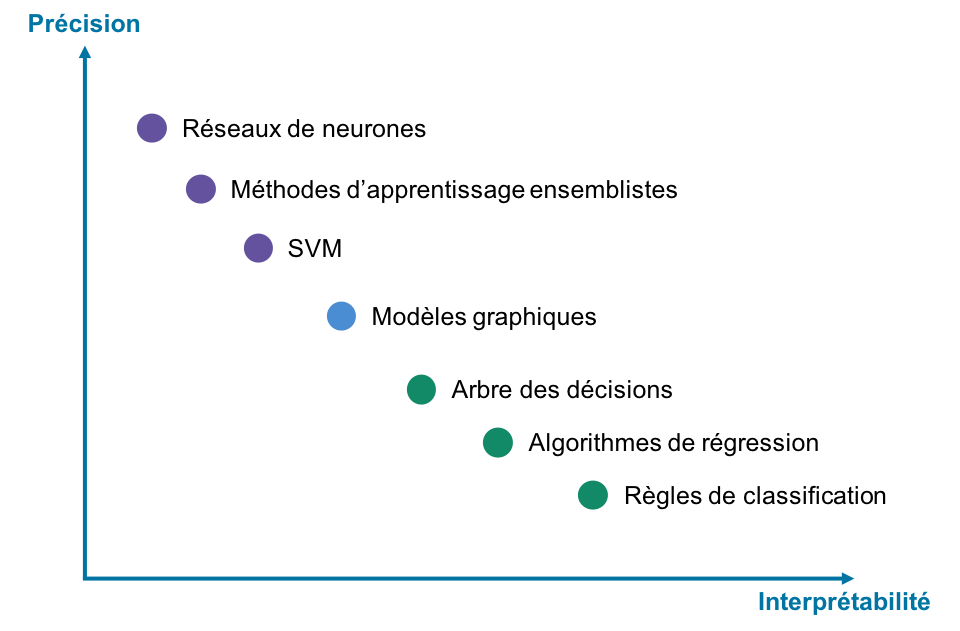
\includegraphics[width= 17 cm]{./figures/acc_vs_int.png}
    \caption{}
\end{figure}

Nous faisons le choix de comparer deux modèles aux performances jugées différentes : l'une est une méthode d'apprentissage ensembliste (random forest) l'autre un algorithme de régression (méthode k-nn).\par

Nous allons donc dans cette section comparer ces 2 méthodes.







%------------------------------------------------------%
\subsection{Méthode 1 : Méthode random forest}
%------------------------------------------------------%

\textbf{Paramètres et implémentation :} \\


Dans le cadre de notre étude nous utulisons l'objet RandomForestClassifier. Ses paramètres les plus importants sont :
\begin{itemize}
    \item max\_features correspond aux nombres de features/attributs à chaque split
    \item n\_estimators correspond aux nombres d'arbres. C'est un paramètre de type entier. Il est égale à 10 par défaut.
    \item max\_samples : taille de l'échantillon aléatoire tiré de la base d'apprentissage
    \item min\_samples\_leaf : correspond au nombre minimal d'éléments  dans un noeud.
    \item oob\_score : correspond à l'estimation ou non de l’erreur de généralisation OOB (Out of Bag).
\end{itemize}

%------------------------------------------------------%
\subsection{Méthode 2 : Méthode des k plus proches voisins (k-nearest neighbors algorithm)}
%------------------------------------------------------%

%------------------------------------------------------%
%------------------------------------------------------%
\section{Annexe}
%------------------------------------------------------%
%------------------------------------------------------%

\newpage
\printbibliography[
heading=bibintoc,
] %Prints the entire bibliography with the title "Whole bibliography"

\end{document}
